%%% LaTeX-Vorlage Version 2.1 %%%

% TODO: individuelle Einstellungen (Name, Titel etc.)
% -> bitte in Konfigurationsdatei anpassen
%%%%
%
% Zentrale Konfigurationsdatei
%
% In dieser Datei sind eine Reihe verpflichtender Einstellungen 
% (Nr. 1 bis 6) vorzunehmen.
%
% Die Einstellungen unter Nr. 7 bis 11 können im Regelfall unverändert
% belassen werden. Ausnahmen sind:
%  - Ihre Arbeit ist in englischer Sprache verfasst (Nr. 7)
%  - der Titel Ihrer Arbeit ist sehr lang, so dass er nicht auf das
%    Deckblatt passt oder anders umgebrochen werden soll (Nr. 8 und 9)
%  - es soll ein besonderes Abgabedatum angegeben werden (Nr. 10)
%  - Sie benötigen einen Vertraulichkeitsvermerk (Nr. 11)
%
%%%%


% TODO 1. Typ der Arbeit (für Titelseite und Metadaten)
% Zutreffendes auswählen:

%\newcommand{\typMeinerArbeit}{PA1} 
\newcommand{\typMeinerArbeit}{PA2} 
%\newcommand{\typMeinerArbeit}{Seminararbeit} 
%\newcommand{\typMeinerArbeit}{BA} 

% TODO 2. Vorname, Name der Autorin/des Autors (für Deckblatt und Metadaten)
\newcommand{\meinName}{Jo Imping}

% TODO 3. Kurs eintragen
\newcommand{\meinKurs}{WWI2023A}

% TODO 4. Titel der Arbeit (für Deckblatt, ehrenwörtliche Erklärung und Metadaten, ohne Umbrüche angeben)
\newcommand{\themaMeinerArbeit}{Fahrzeugbalance-Vorhersage im Motorsport: Entwicklung und Evaluation von Gradient-Boosting-Modellen auf Basis von Porsche LMDh Telemetriedaten}

% TODO 5. Angaben zum Unternehmen (wird bei Seminararbeiten nicht angezeigt)
\newcommand{\UNName}{Dr. Ing. h.c. F. Porsche AG}
\newcommand{\UNBetreuer}{Paul, Stiegele}
\newcommand{\UNBetreuerFunktion}{IT Product Manager}

% TODO 6. Angaben zur wissenschaftlichen Betreuung 
\newcommand{\DHBWBetreuer}{Prof. Dr. Alexander Brandt}


% OPTIONALE Einstellungen

% 7. Arbeit in Englisch
% (nur ändern, falls Ihre Arbeit in englischer Sprache geschrieben ist)
\newcommand{\meineSprache}{DE}	% Standard-Einstellung
%\newcommand{\meineSprache}{EN}	% für Arbeiten in englischer Sprache

% 8. Schriftgröße des Titels auf Deckblatt
% (nur ändern, falls Sie einen sehr langen Titel haben)
% Zutreffendes auswählen:
%\newcommand{\schriftgroesseTitel}{\LARGE}   % Standard-Einstellung
\newcommand{\schriftgroesseTitel}{\Large}  % bei sehr langen Titeln

% 9. Titel mit Umbrüchen für Deckblatt
% (nur ändern, falls Sie den Zeilenumbruch selbst beeinflussen möchten)
\newcommand{\titelAufDeckblatt}{\themaMeinerArbeit}		% Standard-Einstellung
%\newcommand{\titelAufDeckblatt}{Herausforderungen der Digitalisierung im globalen Wettbewerb von Industrieunternehmen \\ -- eine vergleichende Untersuchung unter Berücksichtigung aktueller und weniger aktueller Forschungsmethoden \\ am Beispiel der Firma Melanie Müller und Söhne AG} % explizite Angabe

% 10. Abgabedatum anpassen
% Zutreffendes auswählen:
\newcommand{\abgabeDatum}{24.11.2025}  		% Standard-Einstellung
%\newcommand{\abgabeDatum}{TT.MM.JJJJ}  % falls nicht aktuelles Datum

% 11. Vertraulichkeitsvermerk
% (nur ändern, falls Ihre Arbeit einen Vertraulichkeitsvermerk tragen soll)
\newcommand{\hatVermerk}{nein}  	% Standard-Einstellung
% \newcommand{\hatVermerk}{ja}  	% falls Vertraulichkeitsvermerk


% Grundlegende Dokumenteneigenschaften gemäß DHBW-Vorgaben
\documentclass[a4paper,fontsize=11pt,oneside,parskip=half,headings=normal,listof=nochaptergap]{scrreprt} 
% \usepackage{showframe} % nur für Kontrolle der Ränder 
\usepackage{float}
\usepackage[left]{lineno}
\usepackage{pdfpages}
%%% Präambel einbinden (mit Festlegungen gemäß DHBW-Vorgaben) %%%
%%% Präambel %%%
% hier sollten keine Änderungen erforderlich sein
%
\usepackage{ifthen}           % für Umschaltung DE/EN
\newcommand{\DEoEN}[2]{\ifthenelse{\equal{\meineSprache}{DE}}{#1}{#2}}


\usepackage[utf8]{inputenc}   % Zeichencodierung UTF-8 für Eingabe-Dateien
\usepackage[T1]{fontenc}      % Darstellung von Umlauten im PDF

\usepackage{listings}         % für Einbindung von Code-Listings
\lstset{numbers=left,numberstyle=\tiny,numbersep=5pt,texcl=true}
\lstset{literate=             % erlaubt Sonderzeichen in Code-Listings 
{Ö}{{\"O}}1
{Ä}{{\"A}}1
{Ü}{{\"U}}1
{ß}{{\ss}}2
{ü}{{\"u}}1
{ä}{{\"a}}1
{ö}{{\"o}}1
{€}{{\euro}}1
}

\usepackage[
  inner=35mm,outer=15mm,top=25mm,
  bottom=20mm,foot=12mm,includefoot
]{geometry}                 % Einstellungen für Ränder

\DEoEN{
  \usepackage[ngerman]{babel} % Spracheinstellungen Deutsch
  \usepackage[babel,german=quotes]{csquotes} % deutsche Anf.zeichen
}{
 \usepackage[english]{babel} % Spracheinstellungen Englisch
 \usepackage[babel,english=british]{csquotes} % englische Anf.zeichen
}

\usepackage{enumerate}      % anpassbare Nummerier./Aufz.
\usepackage{graphicx}       % Einbinden von Grafiken
\usepackage[onehalfspacing]{setspace} % anderthalbzeilig

\usepackage{blindtext}      % Textgenerierung für Testzwecke
\usepackage{color}          % Verwendung von Farbe 

\usepackage[nohyperlinks]{acronym}        % für ein Abkürzungsverzeichnis

\usepackage[                % Biblatex
  backend=biber,
  bibstyle=_dhbw_authoryear,maxbibnames=99,
  citestyle=authoryear, dashed=false,    
  uniquename=true, useprefix=true,
  bibencoding=utf8]{biblatex}
%kein Punkt am Ende bei \footcite
%http://www.golatex.de/footcite-ohne-punkt-am-schluss-t4865.html
\renewcommand{\bibfootnotewrapper}[1]{\bibsentence#1}

% Bibliographie: Vornamen ausgeschrieben
\DeclareNameAlias{author}{family-given}
\DeclareNameAlias{editor}{family-given}

%Reihenfolge der Autorennamen
%   
% http://golatex.de/viewtopic,p,80448.html#80448
% Argumente: siehe http://texwelt.de/blog/modifizieren-eines-biblatex-stils/
\DeclareNameFormat{sortname}{% Bibliographie
  \ifnum\value{uniquename}=0 % Normalfall
    \ifuseprefix%
      {%
         \usebibmacro{name:family-given}
           {\namepartfamily}
           {\namepartgiveni}
           {\namepartprefix}
           {\namepartsuffixi}%
       }
      {%
         \usebibmacro{name:family-given}
           {\namepartfamily}
           {\namepartgiveni}
           {\namepartprefixi}
           {\namepartsuffixi}%
       }%
  \fi
  \ifnum\value{uniquename}=1% falls nicht eindeutig, abgek. Vorname 
      {%
         \usebibmacro{name:family-given}
           {\namepartfamily}
           {\namepartgiveni}
           {\namepartprefix}
           {\namepartsuffix}%
       }%
  \fi
  \ifnum\value{uniquename}=2% falls nicht eindeutig, ganzer Vorname 
      {%
         \usebibmacro{name:family-given}
           {\namepartfamily}
           {\namepartgiven}
           {\namepartprefix}
           {\namepartsuffix}%
       }%
  \fi   
  \usebibmacro{name:andothers}}

\DeclareNameFormat{labelname}{% für Zitate
  \ifnum\value{uniquename}=0 % Normalfall
    \ifuseprefix%
      {%
         \usebibmacro{name:family-given}
           {\namepartfamily}
           {\empty}
           {\namepartprefix}
           {\namepartsuffixi}%
       }
      {%
         \usebibmacro{name:family-given}
           {\namepartfamily}
           {\empty}
           {\namepartprefixi}
           {\namepartsuffixi}%
       }%
  \fi
  \ifnum\value{uniquename}=1% falls nicht eindeutig, abgek. Vorname 
      {%
         \usebibmacro{name:family-given}
           {\namepartfamily}
           {\namepartgiveni}
           {\namepartprefix}
           {\namepartsuffix}%
       }%
  \fi
  \ifnum\value{uniquename}=2% falls nicht eindeutig, ganzer Vorname 
      {%
         \usebibmacro{name:family-given}
           {\namepartfamily}
           {\namepartgiven}
           {\namepartprefix}
           {\namepartsuffix}%
       }%
  \fi   
  \usebibmacro{name:andothers}}
      
  
\DeclareFieldFormat{extrayear}{% = the 'a' in 'Jones 1995a'
  \iffieldnums{labelyear}
    {\mknumalph{#1}}
    {\mknumalph{#1}}}        

% Namen getrennt durch Komma (Zitate)
\DeclareDelimFormat*[footcite,cite,textcite,parencite]{multinamedelim}{\addcomma\space}
% bzw. Semikolon (Literaturverzeichnis)
\DeclareDelimFormat[bib,biblist]{multinamedelim}{\addsemicolon\space}
% keine besondere Behandlung beim letzten Autor
\DeclareDelimAlias{finalnamedelim}{multinamedelim}
%\DeclareDelimAlias{multilistdelim}{multinamedelim}

\renewcommand{\nameyeardelim}{~}

% Literaturverzeichnis: Doppelpunkt zwischen Name (Jahr): Rest 
% http://de.comp.text.tex.narkive.com/Tn1HUIXB/biblatex-authoryear-und-doppelpunkt
\renewcommand{\labelnamepunct}{\addcolon\addspace}

% damit die Darstellung für Vollzitate von Primärquellen in 
% Fußnoten später auf "nicht fett" geändert werden kann 
% (nur für Zitate von Sekundärliteratur relevant)
\newcommand{\textfett}[1]{\textbf{#1}}

% für Zitate von Sekundärliteratur:
\newcommand{\footcitePrimaerSekundaer}[4]{%
  \renewcommand{\textfett}[1]{##1}%
  \footnote{\fullcite[#2]{#1}, \DEoEN{zitiert nach}{as cited in} \cite[#4]{#3}}%  
  \renewcommand{\textfett}[1]{\textbf{##1}}%
}

% Im Literaturverzeichnis: Autor (Jahr) fett
\renewbibmacro*{author}{%
  \ifboolexpr{%
    test \ifuseauthor%
    and
    not test {\ifnameundef{author}}
  }
    {\usebibmacro{bbx:dashcheck}
       {\bibnamedash}
       {\usebibmacro{bbx:savehash}%
        \textfett{\printnames{author}}%
        \iffieldundef{authortype}
          {\setunit{\addspace}}
          {\setunit{\addcomma\space}}}%
     \iffieldundef{authortype}
       {}
       {\usebibmacro{authorstrg}%
        \setunit{\addspace}}}%
    {\global\undef\bbx@lasthash
     \usebibmacro{labeltitle}%
     \setunit*{\addspace}}%
  \textfett{\usebibmacro{date+extrayear}}}

% Sonderfall: Quelle ohne Autor, aber mit Herausgeber
% Name des Herausgebers wird fett gedruckt
\renewbibmacro*{bbx:editor}[1]{%
  \ifboolexpr{%
    test \ifuseeditor%
    and
    not test {\ifnameundef{editor}}
  }
    {\usebibmacro{bbx:dashcheck}
       {\bibnamedash}
       {\textfett{\printnames{editor}}%
        \setunit{\addcomma\space}%
        \usebibmacro{bbx:savehash}}%
     \usebibmacro{#1}%
     \clearname{editor}%
     \setunit{\addspace}}%
    {\global\undef\bbx@lasthash
     \usebibmacro{labeltitle}%
     \setunit*{\addspace}}%
  \textfett{\usebibmacro{date+extrayear}}}

\DefineBibliographyStrings{ngerman}{% Anpassungen für deutsche Sprache
	nodate = {{o.J.}},
	urlseen = {{Abruf:}},
	ibidem = {{ebenda}},
	andothers = {{et\addabbrvspace al\adddot}}
}
\DefineBibliographyStrings{english}{% Anpassungen für englische Sprache
    nodate = {{w.y.}},
    urlseen = {{retrieval:}}
}

% keine Anführungszeichen beim Titel im Literaturverzeichnis
\DeclareFieldFormat[article,book,inbook,inproceedings,manual,misc,phdthesis,thesis,online,report]{title}{#1\isdot}

\newcommand{\literaturverzeichnis}{%
% nur Literaturverzeichnis
% (als eigenes Kapitel)
\phantomsection
\addcontentsline{toc}{chapter}{\refname}
\spezialkopfzeile{\refname}
\defbibheading{lit}{\chapter*{\refname}}
\label{chapter:quellen}
\nocite{*} % Alle Einträge der Bibliographie anzeigen, auch unzitierte
\printbibliography[heading=lit,notkeyword=ausblenden]
}
 % mit DHBW-spezifischen Einstellungen

\usepackage{tocloft}        % für Verzeichnis der Anhänge

\usepackage{multirow}       % Tabellenformatierung 

\usepackage{amsmath}        % Erweiterung math. Formelsatz
\usepackage{amssymb}        % math. Symbole

\usepackage{booktabs}       % professionelle Tabellen

\usepackage[hypertexnames=false]{hyperref}       % URL-Formatierung, klickbare Verweise

% Anhänge
\newcounter{anhcnt}
\setcounter{anhcnt}{0}
\newlistof{anhang}{app}{}

\newcommand{\anhang}[1]{%
  \refstepcounter{anhcnt}
  \setcounter{anhteilcnt}{0}
  \section*{\appendixname\ \theanhcnt: #1}
  \addcontentsline{app}{section}{\protect\numberline{\appendixname\ \theanhcnt}#1}\par
}

\newcounter{anhteilcnt}
\setcounter{anhteilcnt}{0}

\newcommand{\anhangteil}[1]{%
	\refstepcounter{anhteilcnt}
	\subsection*{\appendixname\ \arabic{anhcnt}/\arabic{anhteilcnt}: #1}
	\addcontentsline{app}{subsection}{\protect\numberline{\appendixname\ \theanhcnt/\arabic{anhteilcnt}}#1}\par
}

\renewcommand{\theanhteilcnt}{\appendixname\ \theanhcnt/\arabic{anhteilcnt}}

% vgl. S. 4 Paket-Beschreibung tocloft 	
% Einrückungen für Anhangverzeichnis
\makeatletter
\newcommand{\abstaendeanhangverzeichnis}{
\renewcommand*{\l@section}{\@dottedtocline{1}{0em}{5.5em}}
\renewcommand*{\l@subsection}{\@dottedtocline{2}{2.3em}{6.5em}}
}
\makeatother

% Einrückungen
\makeatletter
\renewcommand*{\l@figure}{\@dottedtocline{1}{0em}{2.3em}}
\renewcommand*{\l@table}{\@dottedtocline{1}{0em}{2.3em}}
\makeatother


\usepackage{chngcntr}                % fortlaufende Zähler für Fußnoten, Abbildungen und Tabellen
\counterwithout{figure}{chapter}
\counterwithout{table}{chapter}
\counterwithout{footnote}{chapter}

\usepackage[automark]{scrlayer-scrpage} 
%% Definitionen für Kopf- und Fußzeile auf normalen Seiten
\defpagestyle{kopfzeile}
{% Kopfdefinition
  (\textwidth,0pt)    % Länge der oberen Linie,Dicke der oberen Linie       
  {} % Definition für linke Seiten im doppelseitigen Layout
  {} % Definition für rechte Seiten im doppelseitigen Layout      
  {  % Definition für Seiten im einseitigen Layout
	\makebox[0pt][l]{\rightmark}% 
	\makebox[\linewidth]{}% 
  }        
  (\textwidth, 0.4pt) % Untere Linienlänge, Untere Liniendicke
}
{% Fußdefinition
  (\textwidth,0pt)    % Obere Linienlänge, Obere Liniendicke
  {} % Definition für linke Seiten im doppelseitigen Layout
  {} % Definition für rechte Seiten im doppelseitigen Layout
  {  % Definition für Seiten im einseitigen Layout
    \makebox[\linewidth]{}%
    \makebox[0pt][r]{\pagemark}%
  }
  (\textwidth, 0pt)   % Länge der unteren Linie,Dicke der unteren Linie
}

%% Definitionen für Kopf- und Fußzeile auf ersten Seiten eines Kapitels
\defpagestyle{kapitelkopfzeile}
{% Kopfdefinition
  (\textwidth,0pt)    % Länge der oberen Linie,Dicke der oberen Linie       
  {} % Definition für linke Seiten im doppelseitigen Layout
  {} % Definition für rechte Seiten im doppelseitigen Layout      
  {}  % Definition für Seiten im einseitigen Layout
  (\textwidth, 0pt) % Untere Linienlänge, Untere Liniendicke
}
{% Fußdefinition
  (\textwidth,0pt)    % Obere Linienlänge, Obere Liniendicke
  {} % Definition für linke Seiten im doppelseitigen Layout
  {} % Definition für rechte Seiten im doppelseitigen Layout
  {  % Definition für Seiten im einseitigen Layout
    \makebox[\linewidth]{}%
    \makebox[0pt][r]{\pagemark}%
  }
  (\textwidth, 0pt)   % Länge der unteren Linie,Dicke der unteren Linie
}

%% Definitionen für Kopf- und Fußzeile im Anhang und bei Quellenverzeichnisse
\newcommand{\spezialkopfzeileBezeichnung}{}
\defpagestyle{spezialkopfzeile}
{% Kopfdefinition
  (\textwidth,0pt)    % Länge der oberen Linie,Dicke der oberen Linie       
  {} % Definition für linke Seiten im doppelseitigen Layout
  {} % Definition für rechte Seiten im doppelseitigen Layout      
  {  % Definition für Seiten im einseitigen Layout
	\makebox[0pt][l]{\spezialkopfzeileBezeichnung}% 
	\makebox[\linewidth]{}% 
  }        
  (\textwidth, 0.4pt) % Untere Linienlänge, Untere Liniendicke
}
{% Fußdefinition
  (\textwidth,0pt)    % Obere Linienlänge, Obere Liniendicke
  {} % Definition für linke Seiten im doppelseitigen Layout
  {} % Definition für rechte Seiten im doppelseitigen Layout
  {  % Definition für Seiten im einseitigen Layout
    \makebox[\linewidth]{}%
    \makebox[0pt][r]{\pagemark}%
  }
  (\textwidth, 0pt)   % Länge der unteren Linie,Dicke der unteren Linie
}
            
\newcommand\spezialkopfzeile[1]{%
  \renewcommand\spezialkopfzeileBezeichnung{#1}
  \pagestyle{spezialkopfzeile}
}
                
% Standard-Pagestyle auswählen
\pagestyle{kopfzeile}

% keine Kopfzeile anzeigen auf Seiten, auf denen ein 
% Kapitel beginnt oder das Inhalts-/Abbildungs-/Tabellenverzeichnis steht 
\renewcommand{\chapterpagestyle}{kapitelkopfzeile}
\tocloftpagestyle{kapitelkopfzeile}

		 % für schöne Kopfzeilen 

\usepackage{textcomp}            % erlaubt EUR-Zeichen in Eingabedatei
\usepackage{eurosym}             % offizielles EUR-Symbol in Ausgabe
\renewcommand{\texteuro}{\euro}  % ACHTUNG: nach hyperref aufrufen!

\usepackage{scrhack}             % stellt Kompatibilität zw. KOMA-Script
                                 % (scrreprt) und anderen Paketen her
                                 
% Anpassung der Abstände bei Kapitelüberschriften
% (betrifft auch Inhalts-, Abbildungs- und Tabellenverzeichnis)
\renewcommand*\chapterheadstartvskip{\vspace*{-\topskip}}
\newcommand{\myBeforeTitleSkip}{1mm}
\newcommand{\myAfterTitleSkip}{10mm}
\setlength\cftbeforetoctitleskip{\myBeforeTitleSkip}
\setlength\cftbeforeloftitleskip{\myBeforeTitleSkip}
\setlength\cftbeforelottitleskip{\myBeforeTitleSkip}

\setlength\cftaftertoctitleskip{\myAfterTitleSkip}
\setlength\cftafterloftitleskip{\myAfterTitleSkip}
\setlength\cftafterlottitleskip{\myAfterTitleSkip}

% Anhang beginnen
\newcommand{\startAnhang}{%
\chapter*{\appendixname}
\addcontentsline{toc}{chapter}{\appendixname}
\section*{\anhangVzBezeichnung}
\vspace{-8em}

% vor \listofanhang müssen Einrückungen angepasst werden
\abstaendeanhangverzeichnis
\spezialkopfzeile{\DEoEN{Anhang}{Appendix}} % damit in der Kopfzeile das Wort "Anhang" angezeigt wird
}

% Abkürzungsverzeichnis beginnen
\newcommand{\startAbkVerzeichnis}{%
\chapter*{\abkVzBezeichnung}
\addcontentsline{toc}{chapter}{\abkVzBezeichnung}
}

% einfaches Umstellen der Zeilenabstände in Tabellen
\newcommand{\ra}[1]{\renewcommand{\arraystretch}{#1}}


% Sprach-spezifische Einstellungen
\DEoEN{%
\newcommand{\abkVzBezeichnung}{Abkürzungsverzeichnis}
\newcommand{\anhangVzBezeichnung}{Anhangverzeichnis}

\renewcaptionname{ngerman}{\refname}{Literaturverzeichnis} % statt "Literatur"
\renewcaptionname{ngerman}{\figurename}{Abb.}
\renewcaptionname{ngerman}{\tablename}{Tab.}
}{
\newcommand{\abkVzBezeichnung}{Abbreviations}
\newcommand{\anhangVzBezeichnung}{Appendix directory}

\renewcaptionname{english}{\contentsname}{Table of Contents}
\renewcaptionname{english}{\figurename}{Fig.}
\renewcaptionname{english}{\tablename}{Tab.}
}


                                                            
%%% Ende der Präambel %%%

%%% Name der eigenen Literatur-Datenbank (ggf. anpassen) %%%
\bibliography{includes/literatur-datenbank.bib}


\begin{document}
%%% Deckblatt gemäß DHBW-Vorgaben einbinden (keine Anpassung nötig) %%% 
% 
% in dieser Datei sind keine Anpassungen nötig
%
% alle erforderlichen Festlegungen treffen Sie in config.tex
%
\thispagestyle{empty}

\begin{spacing}{1}
\begin{center}	
~\vspace{0mm}

{\sffamily
\schriftgroesseTitel  
\textbf{\titelAufDeckblatt}
}


\vspace{15mm}

{\Large%
\DEoEN{%
  \ifthenelse{\equal{\typMeinerArbeit}{PA1}}{1. Projektarbeit}{}%
  \ifthenelse{\equal{\typMeinerArbeit}{PA2}}{2. Projektarbeit}{}%
  \ifthenelse{\equal{\typMeinerArbeit}{BA}}{Bachelorarbeit}{}%
  \ifthenelse{\equal{\typMeinerArbeit}{Seminar}}{Seminararbeit}{}%
}{% 
  \ifthenelse{\equal{\typMeinerArbeit}{PA1}}{1. Project work}{}%
  \ifthenelse{\equal{\typMeinerArbeit}{PA2}}{2. Project work}{}%
  \ifthenelse{\equal{\typMeinerArbeit}{BA}}{Bachelor thesis}{}%
  \ifthenelse{\equal{\typMeinerArbeit}{Seminar}}{Seminar work}{}%
}}

\vspace{1cm}

\DEoEN{vorgelegt am}{submitted on} \abgabeDatum 

\vspace{15mm}

\DEoEN{Fakultät Wirtschaft und Gesundheit}{Faculty of Economics and Health} 

\medskip
\DEoEN{Studiengang Wirtschaftsinformatik}{Business informatics degree programme}

\medskip

\DEoEN{Kurs}{Course} \meinKurs 

\vspace{10mm}

\DEoEN{von}{by}

\vspace{10mm}

{\large\textsc{\meinName}}

\vspace{10mm}
\end{center}

\vfill

\begin{tabular}{ll}
\DEoEN{Betreuung in der Ausbildungsstätte:}{Responsible person in the training centre:}
& DHBW Stuttgart: \\
\hspace{0.45\linewidth} & \\
\UNName & \multirow[t]{2}{*}{\DHBWBetreuer} \\
\UNBetreuer & \\
\UNBetreuerFunktion & \\
\\
\DEoEN{Unterschrift}{Signature} \\
\end{tabular}

\vspace{1cm}
\end{spacing}

\ifthenelse{\equal{\hatVermerk}{ja}}{%
\begin{center}
\small
\DEoEN{%
\textbf{Vertraulichkeitsvermerk}:
Der Inhalt dieser Arbeit darf weder als Ganzes noch in Auszügen \\
Personen außerhalb des Prüfungs- und Evaluationsverfahrens zugänglich gemacht werden, \\ sofern keine anders lautende Genehmigung des Dualen Partners vorliegt.%
}{%
\textbf{Confidentiality notice}:
The content of this work may not be made accessible to people outside \\ of the testing process and the evaluation process neither as a whole nor as excerpts, unless an authorisation stating otherwise is presented by the training facility.%
}
\end{center}%
}{}

% Meta-Daten für PDF-Datei basierend auf obigen Angaben
\hypersetup{pdftitle={\themaMeinerArbeit}}
\hypersetup{pdfauthor={\meinName}}
\hypersetup{pdfsubject={\typMeinerArbeit\ DHBW Stuttgart \the\year}}
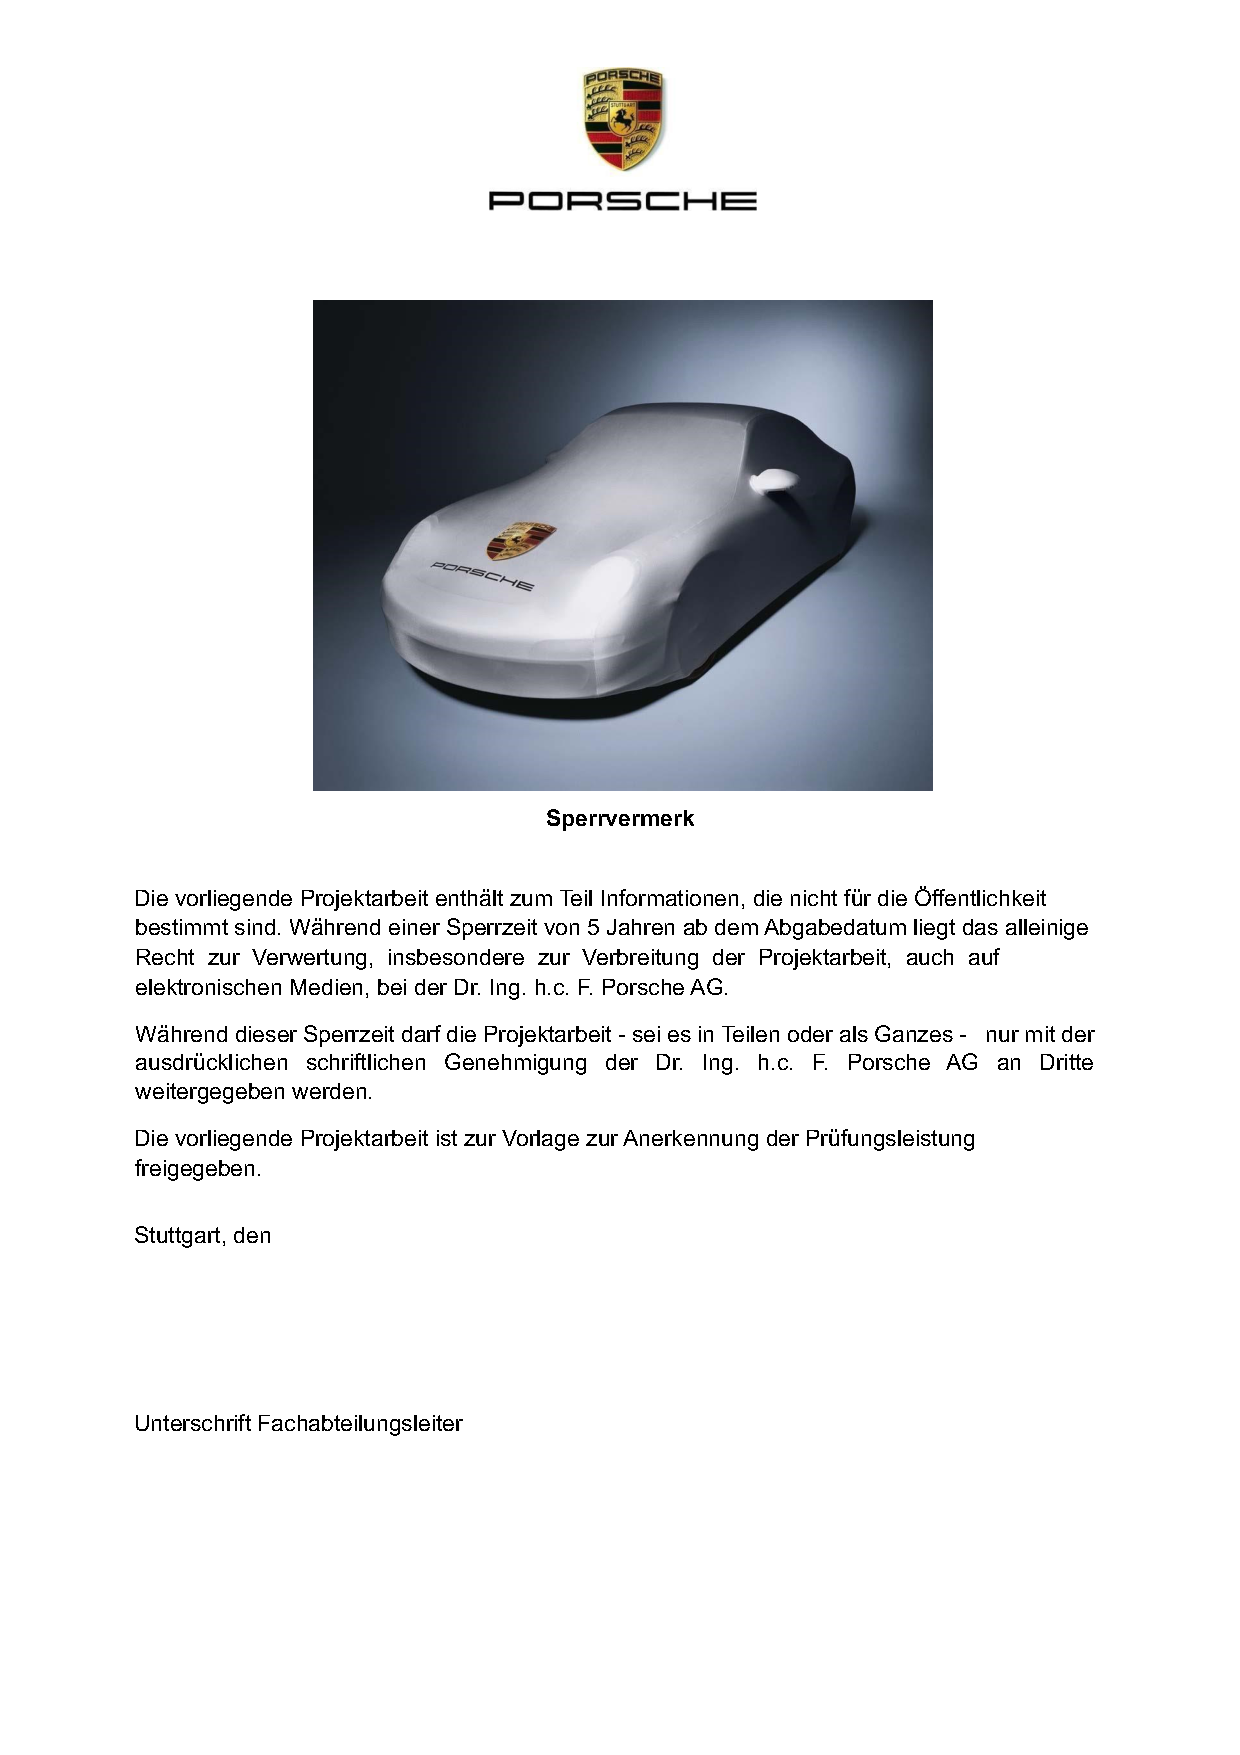
\includepdf[pages=1]{includes/Sperrvermerk_Abschlussarbeit.pdf}

%%% Umstellung der Seiten-Nummerierung auf i, ii, iii ... %%%
\pagenumbering{Roman} 


%%% Inhalts-, Abbildungs-, Tabellenverzeichnisse %%%
% werden einzeilig gesetzt, um Platz zu sparen 
\begin{spacing}{1}
\tableofcontents % Inhaltsverzeichnis ausgeben
\clearpage
\startAbkVerzeichnis


\begin{acronym}[DHBW] 
% Argument definiert die Breite der ersten Spalte anhand des längsten vorkommenden Eintrags
\acro{DSR}{Design Science Research}
\acro{EDA}{Explorative Datenanalyse}
\acro{GBDT}{Gradient Boosting Decision Trees}
\acro{KQL}{Kusto Query Language}
\acro{ML}{Machine Learning}
\acro{MAE}{Mean Absolute Error}
\acro{RMSE}{Root Mean Squared Error}
\acro{SVR}{Support Vector Regression}
\acro{IMSA}{International Motor Sports Association}
\acro{WEC}{World Endurance Championship}


\end{acronym}

 % Abkürzungsverzeichnis einbinden

\clearpage
\thispagestyle{kapitelkopfzeile}
\listoffigures
\phantomsection
\addcontentsline{toc}{chapter}{\listfigurename} % Abb.verz. ins Inh.verz. aufnehmen

\clearpage
\listoftables
\phantomsection
\addcontentsline{toc}{chapter}{\listtablename} % Tab.verz. ins Inh.verz. aufnehmen
\end{spacing}

%%% Umstellung der Seiten-Nummerierung auf 1, 2, 3 ... %%%
\cleardoublepage
\pagenumbering{arabic}

%%% Ihr eigentlicher Inhalt %%%
% Empfehlung: strukturieren Sie Ihren Text in einzelnen Dateien 
% und binden Sie diese hier mit \input{includes/dateiname.tex} ein
\chapter{Einleitung}

\textbf{Einführung Motorsport bei Porsche}

\section{Problemstellung und Motivation}
Im Rennsport hängt die Fahrzeugbalance von zahlreichen, komplex miteinander verflochtenen Einflussgrößen, sodass Ingenieure aktuell nicht nachvollziehen können, welche Kombinationen dieser Parameter eine Balance-Änderung hervorrufen, und daher erst reaktiv handeln, wenn Abweichungen auftreten. Ziel ist es, zu verstehen, wie diese Einflussgrößen gemeinsam die Fahrzeugbalance steuern, um proaktiv fundierte Entscheidungen treffen zu können.

\section{Zielsetzung und Forschungsfragen}

Ziel dieser Arbeit ist es zunächst, ein maschinelles Lernmodell zu entwickeln, das auf Basis der Parameter  
\textit{Tracktemperatur, Reifentemperatur, Reifendruck, Fahrertyp, Mechanical Balance (Anti-Roll-Bar-Front/Rear),}  
\textit{Reifenmischung, Reifenmileage, Softwareeinstellungen (Brake Balance, Traktionskontrolle)} und  
\textit{Kraftstoffgewicht} die Fahrzeugbalance mit hoher Genauigkeit vorhersagt. Darauf aufbauend wird  
mittels Explainable AI untersucht, wie diese Einflussgrößen gemeinsam die Zielvariable determinieren,  
um Ingenieuren ein Verständnis der wirkenden Zusammenhänge zu ermöglichen.

\paragraph{Forschungsfragen}
\begin{enumerate}
  \item Lässt sich ein ML-Modell konstruieren, das die Fahrzeugbalance zuverlässig prognostiziert?
  \item Können Explainable-AI-Methoden wertvolle Einblicke darin liefern, wie die betrachteten Einflussfaktoren gemeinsam die Fahrzeugbalance bestimmen?
\end{enumerate}


\section{Aufbau der Arbeit}
Die vorliegende Arbeit ist so strukturiert, dass beide Forschungsfragen systematisch beantwortet werden. 

In Kapitel 2 werden zunächst die relevanten theoretischen Grundlagen vermittelt. Abschnitt 2.1 führt in die Design-Science-Research-Methodologie ein, mit der Frage 1 (Entwicklung eines Vorhersagemodells) begleitet wird. Abschnitt 2.2 beschreibt die Grundlagen zu maschinellen Lernverfahren für Regression und insbesondere XGBoost, die später in Kapitel 4 zur Realisierung des Modells eingesetzt werden. Abschnitt 2.3 gibt einen kompakten Überblick zu Explainable-AI-Techniken, die in Kapitel 7 zur Beantwortung von Frage 2 (Erkenntnisgewinn mittels Explainable AI) relevant sind.

Kapitel 3 widmet sich der Anforderungsanalyse und Problemdefinition im DSR Relevance Cycle. Hier werden die fachlichen, funktionalen und nicht-funktionalen Anforderungen abgeleitet, die notwendig sind, um Frage 1 zu beantworten: Die Festlegung von Zielgrößen wie \(R^2\ge0{,}85\) und die Varianz-Abdeckung durch die Top-10-Features sichert die Modellqualität.

Kapitel 4 beschreibt das Design und die Implementierung des Vorhersagemodells (DSR Design \& Build Cycle). Dabei werden die Datenpipeline, das Training mit XGBoost und das Hyperparameter-Tuning detailliert dargestellt, um Frage 1 praktisch umzusetzen.

Kapitel 5 enthält die Evaluation des trainierten Modells (DSR Rigor Cycle). Quantitative Metriken wie R², RMSE und die kumulierte Varianz-Erklärung durch die Top-10-Features werden ausgewertet, um abschließend zu bestätigen, dass Frage 1 erfüllt ist.

Kapitel 6 reflektiert das Modell-Artefakt und zieht Lessons Learned aus dem Entwicklungsprozess. Hier werden Design-Entscheidungen und Einschränkungen kritisch beleuchtet, bevor der Fokus auf Frage 2 wechselt.

Kapitel 7 ist dem Erkenntnisgewinn mittels Explainable AI gewidmet. Mit SHAP-Analysen und weiteren Interpretationsmethoden wird Frage 2 beantwortet: Es wird aufgezeigt, wie die betrachteten Einflussfaktoren gemeinsam die Fahrzeugbalance bestimmen und welche praktischen Einsichten Ingenieuren damit zur Verfügung stehen.

Kapitel 8 fasst die Ergebnisse zusammen, beantwortet nochmals beide Forschungsfragen und gibt einen Ausblick auf mögliche weiterführende Arbeiten. Zudem enthält es eine kritische Selbsteinschätzung des DSR-Prozesses und des erzielten Nutzens.  

\chapter{Theoretische Grundlagen}

Zur Entwicklung eines \ac{ML}-Modells für Motorsport-Telemetrie-Analyse 
müssen mehrere ineinandergreifende Konzepte verstanden werden. Dieses Kapitel 
vermittelt zunächst methodologische Grundlagen (Design Science Research, 
Datenvorverarbeitung), dann die Theorie von Regressionsproblemen und speziell 
Gradient Boosting Decision Trees, und abschließend praktische Aspekte von 
Optimierung und Validierung. Diese Grundlagen bilden die wissenschaftliche Basis 
für die in Kapitel 4 beschriebene Artefakt-Entwicklung.


\section{Design Science Research Methodologie}

\ac{DSR} ist ein etablierter Forschungsansatz der Wirtschaftsinformatik, der sich grundlegend von deskriptiven Forschungsmethoden unterscheidet. Während traditionelle empirische Forschung primär darauf ausgerichtet ist, bestehende Phänomene zu verstehen und zu erklären, zielt \ac{DSR} darauf ab, praktische Probleme durch systematische Entwicklung und rigorose Evaluierung von Artefakten zu lösen. Damit schafft \ac{DSR} eine Brücke zwischen wissenschaftlicher Fundierung und praktischer Problemlösung.\footnote{Vgl. \cite{Hevner2004}, S. 77-83}

Das Grundwerk von Hevner et al. (2004) prägt bis heute das Verständnis von \ac{DSR} und etabliert ein Framework, das auf sieben präskriptiven Richtlinien basiert. Das Framework schreibt vor, dass \ac{DSR}-Projekte in drei ineinandergreifenden Zyklen durchgeführt werden sollten: Der Relevance Cycle beginnt mit Problemidentifikation aus der Anwendungsdomäne; der Rigor Cycle verankert die Entwicklung in wissenschaftlichem Wissen und etablierten Theorien; der Design Cycle orchestriert iterative Phasen von Artefakt-Konzeption, Entwicklung und Evaluierung. Diese drei Zyklen ermöglichen eine systematische und nachvollziehbare Forschungsvorgehensweise, bei der wissenschaftliche Strenge nicht auf Kosten von Praxisrelevanz geht.\footnote{Vgl. \cite{Hevner2004}, S. 77-92}

Der \ac{DSR}-Prozess gliedert sich typischerweise in sechs sequenzielle Phasen. Problem Identification and Motivation beginnt mit der Analyse der Problemdomäne und Begründung ihrer wissenschaftlichen und praktischen Relevanz. Definition of Objectives spezifiziert die Anforderungen, die das entwickelte Artefakt erfüllen muss. In der Design and Development Phase wird das Artefakt konzipiert und prototypisch implementiert. Die Demonstration Phase dokumentiert, dass das Artefakt das Problem tatsächlich lösen kann, typischerweise durch Fallstudien oder kontrollierte Szenarien. Die Evaluation Phase bewertet das Artefakt systematisch gegen die vordefinierten Anforderungen und Ziele. Abschließend erfolgt die Communication Phase, in der Erkenntnisse und Design Knowledge der wissenschaftlichen Gemeinschaft mitgeteilt werden.\footnote{Vgl. \cite{Peffers2007}, S. 45-77} 

Artefakte in \ac{DSR} können verschiedene Formen annehmen. Constructs sind konzeptionelle Vokabularien und Abstraktionen, die Probleme präzise definieren. Models stellen Zusammenhänge und Strukturen in vereinfachter Form dar. Methods sind Algorithmen und systematische Verfahrensweisen zur Problemlösung. Instantiations schließlich sind konkrete Implementierungen oder Prototypen.\footnote{Vgl. \cite{Hevner2004}, S. 80} In \ac{ML}-Projekten ist die Instantiation typischerweise ein trainiertes Modell mit vollständiger Pipeline (Datenvorverarbeitung, Feature Engineering, trainierte Parameter). Die vorliegende Arbeit entwickelt eine Instantiation: ein evaluiertes \ac{ML}-Modell für Fahrzeugbalance-Vorhersage.

Die Evaluierung in \ac{DSR} erfüllt mehrere funktionale Rollen. Sie stellt fest, ob und inwieweit das Artefakt die definierten Anforderungen erfüllt. Sie identifiziert Verbesserungspotenziale für weitere Iterationen. Vor allem trägt sie zur wissenschaftlichen Wissensbasis bei, indem Design Principles und generalisierbare Lessons Learned dokumentiert werden.\footnote{Vgl. \cite{Venable2016}, S. 79–81; vgl. dazu auch \cite{Gregor2007}, 
S. 322–325, sowie \cite{Hevner2004}, 
S. 84–85}
 Bewährte Evaluationsmethoden in \ac{DSR} sind observational (Feldbeobachtung), 
analytical (logische Deduktion und Proof-of-Concept), experimental 
(kontrollierte Experimente mit Baseline-Vergleich), testing (systematische 
Funktionsprüfung) und descriptive (qualitative Bewertung durch Experten).\footnote{Vgl. 
\cite{Hevner2004}, S. 85-86} Für \ac{ML}-Artefakte dominieren 
analytische und experimentelle Evaluationen mittels etablierter Performance-Metriken.\footnote{Vgl. \cite{Friedman2009}, S. 420–430}


\section{Experteninterviews zur Anforderungsermittlung}

Die Anforderungsanalyse in Kapitel 3 basiert auf zwei informellen Gesprächen mit einem erfahrenen Performance Engineer aus dem Porsche Motorsport-Team. Das erste Gespräch fand am 29.08.2025 statt, das zweite am 12.09.2025. Ziel war es, durch offene Diskussion die tägliche Arbeitsweise im Telemetrie-Management nachzuvollziehen, zentrale technische Herausforderungen zu identifizieren und realistische Anforderungen an ein automatisiertes Vorhersagemodell zu formulieren.
Der interviewte Experte agiert als Teamleiter der Performance-Abteilung im Porsche LMDh-Programm und ist verantwortlich für die Fahrzeugentwicklung, Simulationsmodellierung und insbesondere die datenbasierte Optimierung des Rennwagen-Setups während des operativen Betriebs, wodurch er über tiefgehendes, direkt anwendbares Wissen im Telemetrie-Management verfügt.\footnote{Vgl. Experteninterview 1, 29.08.2025, Z. 3-27}

Beide Gespräche folgten einem offenen, exploratorischen Format ohne strukturierten Fragenkatalog, um eine natürliche Konversation zu fördern und implizites Wissen des Experten zugänglich zu machen. Die gewonnenen Erkenntnisse bestätigten, dass die aktuelle Telemetrie-Analyse stark manuell erfolgt und mehrere Stunden pro Rennwochenende erfordert. Dies validierte die Problemrelevanz und leitete die Anforderungsableitung in Kapitel 3.\footnote{Vgl. Experteninterview 1 und 2, dokumentiert in Anhang A.1} 



\section{Maschinelle Lernverfahren für Regressionsprobleme}

\ac{ML} wird allgemein als automatische Induktion von vorhersagenden Modellen aus Daten definiert, ohne dass Algorithmen explizit programmiert werden müssen.\footnote{Vgl. Mitchell 1997, S. 1-2} Im praktischen Kontext bedeutet dies: Ein Lernalgorithmus erhält Trainingsdaten, erkennt Muster in diesen Daten und extrahiert eine verallgemeinerbare mathematische Struktur, die auf neue Daten angewendet werden kann.

Das vorliegende Projekt verfolgt ein Regressionsziel: Vorhersage einer kontinuierlichen Zielvariable (Fahrzeugbalance-Wert) aus einer Menge strukturierter Input-Features (Telemetrie-Metriken). Dies unterscheidet sich von Klassifikation, bei der diskrete Kategorien vorhergesagt werden. Regression ist ein Supervised-Learning-Problem: Jede Trainingsinstanz hat ein bekanntes, korrektes Label (den gemessenen Fahrzeugbalance-Wert), gegen das das Modell seine Vorhersagen abgleichen kann.\footnote{Vgl. Hastie et al. 2009, S. 1-25}

Das zentrale Problem beim Modelllernen wird durch den Bias-Variance Trade-off beschrieben. Ein Modell mit niedriger Komplexität wie lineare Regression hat hohen Bias: Es macht systematisch vereinfachte Vorhersagen, die die tatsächliche nichtlineare Beziehung zwischen Features und Zielvariable nicht erfassen und somit zu Underfitting führen. Umgekehrt weist ein hochkomplexes Modell wie ein überparametrisiertes Polynom hohe Varianz auf: Es memoriert Trainingsrauschen und besondere Trainingsfälle und generalisiert dadurch schlecht auf neue Daten, was als Overfitting bezeichnet wird.\footnote{Vgl. Hastie et al. 2009, S. 23-31} Das Ziel ist ein gutes Gleichgewicht: Ein Modell mit ausreichender Komplexität, um die echte Struktur der Daten zu erfassen, aber nicht so komplex, dass es Zufallsrauschen memoriert.

Die Vorbereitung der Daten ist entscheidend für späteren Erfolg. Exploratory Data Analysis (EDA) untersucht zunächst die Rohverteilungen der Features, identifiziert Korrelationen zwischen Variablen und erkennt potenzielle Ausreißer oder Anomalien.\footnote{Vgl. \cite{Tukey1977}, S. 1–50} Data Cleaning adressiert praktische Datenqualitätsprobleme: fehlende Werte werden behandelt durch Imputation oder Ausschluss, anomale Messwerte werden gefiltert, und sachlogische Schwellwerte werden gesetzt, etwa der Ausschluss von Messungen mit unplausiblen Sensorwerten.\footnote{Vgl. \cite{Chapman2000}, S. 23–28}

Feature Engineering ist der kreative Schritt, in dem Rohdaten in aussagekräftige Prädiktoren transformiert werden. Feature Selection wählt von vielen möglichen Kandidaten diejenigen aus, die am meisten zur Vorhersage beitragen und reduziert dadurch Overfitting sowie Trainingszeit.\footnote{Vgl. Guyon, Elisseeff 2003, S. 1157-1182} Aggregation kombiniert hochkorrelierte Sensoren zu zusammengefassten Features, beispielsweise der Durchschnitt mehrerer Temperatur-Sensoren, um Rauschredundanz zu minimieren.\footnote{Vgl. Guyon, Elisseeff 2003, S. 1157-1182} Encoding wandelt kategoriale Variablen wie Track-Identifikatoren in numerische Repräsentationen um.\footnote{Vgl. \cite{Kuhn2019}, S. 139–170} Für Telemetriedaten ist Zeitreihen-Glättung wie Moving Averages essentiell: Sie reduziert hochfrequentes Sensorrauschen, ohne Trends zu zerstören, und ermöglicht es, echte physikalische Änderungen von Messfehlern zu unterscheiden.\footnote{Vgl. \cite{Box2015}, S. 25–45; vgl. dazu auch \cite{Cleveland1979}, S. 829–836}


Nach der Datenvorbereitung entsteht eine zentrale Designfrage: Welcher Regressionsalgorithmus ist am besten geeignet? Lineare Modelle wie Linear Regression, Ridge und Lasso bieten exzellente Interpretierbarkeit, können aber intrinsisch nur lineare Beziehungen erfassen. Interpretierbarkeit hierbei, dass nachvollzogen werden kann, welche Features wie stark die Vorhersage beeinflussen.\footnote{Vgl. Hastie et al. 2009, S. 58-85} Support Vector Regression nutzt mathematische Tricks, die sogenannten Kernel-Tricks, um implizit nichtlineare Feature-Transformationen durchzuführen, bleibt aber schwer zu interpretieren.\footnote{Vgl. Hastie et al. 2009, S. 290-310} Decision Trees sind intuitiv: Sie partitionieren den Feature-Raum sequenziell anhand scharfer Grenzen, etwa wenn Feature X größer als 5 ist, dann gehe linken Ast. Sie sind robust und können komplexe nichtlineare Muster erfassen, leiden aber unter Overfitting, da ein einzelner Baum Trainingsrauschen memoriert.\footnote{Vgl. Breiman 2001, S. 5-32} Random Forests verbessern einzelne Bäume durch Ensemble-Averaging: Viele verschiedene Bäume werden auf zufällig gestörten Datensätzen trainiert, und ihre Vorhersagen werden gemittelt, was Varianz reduziert und Generalisierung verbessert.\footnote{Vgl. Breiman 2001, S. 5-32} Boosting-Methoden folgen einem anderen Ensemble-Prinzip: Sie trainieren Bäume sequenziell, wobei jeder neue Baum systematisch die Fehler vorheriger Bäume korrigiert.\footnote{Vgl. Friedman 2001, S. 1189-1232} Neuronale Netze können beliebig komplexe Funktionen approximieren und funktionieren gut bei großen Datenmengen, erfordern aber typischerweise mehr Trainingsdaten als traditionelle \ac{ML}-Methoden und sind weniger interpretierbar.\footnote{Vgl. Goodfellow et al. 2016, S. 164-223}

Die Frage stellt sich: Welche Methode eignet sich für das vorliegende Motorsport-Problem mit strukturierten, tabulischen Daten von moderater Größe, in denen konkurrierende komplexe Effekte zwischen Features existieren und Interpretierbarkeit gewünscht ist, um Renningenieure zu unterstützen? Unter diesen Bedingungen haben sich Gradient Boosting Decision Trees als Methode der Wahl etabliert, weil sie nichtlineare Muster erfassen, auf moderaten Datenmengen gut funktionieren und ein gutes Gleichgewicht zwischen Vorhersagegenauigkeit und Interpretierbarkeit bieten.\footnote{Vgl. Chen, Guestrin 2016, S. 785-794}



\section{Gradient Boosting Decision Trees}

Gradient Boosting Decision Trees (GBDT) sind eine Ensemble-Methode, die sequenzielle schwache Lerner, das heißt einfache Decision Trees, zu einem starken Vorhersagemodell kombiniert.\footnote{Vgl. Friedman 2001, S. 1189-1232} Das Kernprinzip ist Residual Learning: Der erste Baum wird auf die Rohdaten trainiert. Der zweite Baum wird trainiert, um die Fehler des ersten Baums vorherzusagen, die sogenannten Residuen. Der dritte Baum korrigiert dann die kombinierten Fehler von Baum 1 und 2, und so weiter. Die finale Vorhersage ergibt sich aus einer gewichteten Summe aller Baum-Ausgaben.

Formalisiert wird dies durch Gradient Descent: Eine Loss-Funktion, typischerweise Mean Squared Error für Regression, quantifiziert, wie schlecht die Vorhersagen sind. Jeder neue Baum wird so konstruiert, dass er in Richtung des negativen Gradienten dieser Loss-Funktion läuft, also gezielt Fehler reduziert.\footnote{Vgl. Friedman 2001, S. 1200-1210} Dieser Gradient-Ansatz führt zu schnellerer Konvergenz als alternatives Ensemble-Averaging.

Warum ist GBDT für Regressionsprobleme bevorzugt? Erstens erfasst es nichtlineare Beziehungen zwischen Features und Zielvariable, was lineare Modelle nicht können. Zweitens funktioniert es auf moderaten Datenmengen gut, im Gegensatz zu neuronalen Netzen. Drittens ist es vergleichsweise schnell zu trainieren. Viertens bietet es Feature-Importance-Schätzungen, die zeigen, welche Telemetrie-Signale am meisten zur Fahrzeugbalance-Vorhersage beitragen.

Zwei prominente Implementierungen konkurrieren: XGBoost (eXtreme Gradient Boosting) ist die ältere Implementierung, seit 2014 verfügbar, und bietet hochoptimierte Algorithmen mit integrierten Regularisierungsmechanismen wie L1- und L2-Penalisierungen, die Overfitting kontrollieren.\footnote{Vgl. Chen, Guestrin 2016, S. 785-794} Sie nutzt Histogram-basiertes Split-Finding: Statt Splits für alle kontinuierlichen Werte zu evaluieren, diskretisiert XGBoost Features in Histogramm-Bins, was zu Geschwindigkeitsvorteil führt. Sie hat native Unterstützung für kategoriale Features, wodurch manuelle Encoding-Schritte entfallen. XGBoost wächst Bäume level-wise: Bei jedem Schritt werden alle Blätter auf derselben Tiefe erweitert.

LightGBM (Light Gradient Boosting Machine) ist eine neuere Implementierung von Microsoft ab 2016, die speziell für Geschwindigkeit auf großen Datensätzen optimiert ist.\footnote{Vgl. \cite{Ke2017}, S. 1-10} Sie verwendet Leaf-wise Wachstum: Statt alle Blätter auf gleicher Tiefe zu halten, erweitert sie bei jedem Schritt das Blatt mit dem höchsten Fehlerreduktionspotenzial, was zu tieferen, schmäleren Bäumen führt. Sie nutzt Gradient-based One-Side Sampling: Trainingsinstanzen mit großen Gradienten, die schlecht vorhergesagten, behalten volle Gewichtung, während Instanzen mit kleinen Gradienten, die gut vorhergesagten, untersampled werden. Sie nutzt Exclusive Feature Bundling: Hochkorrelierte Features werden kombiniert, um Dimensionalität zu reduzieren. Diese Optimierungen machen LightGBM oft schneller, zum Preis leicht erhöhten Overfitting-Risikos.

Empirisch zeigen beide Implementierungen überlegene Performance auf strukturierten tabularen Daten im Vergleich zu tiefen neuronalen Netzen.\footnote{Vgl. \cite{Chen2016}, S. 788-792} Die Wahl zwischen ihnen ist oft pragmatisch: XGBoost für Balance, LightGBM wenn Geschwindigkeit kritisch ist.



\section{Hyperparameter-Optimierung und Modellvalidierung}

Um ein GBDT-Modell zu trainieren, müssen vor dem Training viele Hyperparameter gesetzt werden. Hyperparameter unterscheiden sich fundamental von Modell-Parametern, den internen Gewichten des Modells, die während Training gelernt werden. Hyperparameter sind konfigurierbare Knöpfe, die Architekt oder Architektin des Modells kontrolliert.\footnote{Vgl. Bergstra, Bengio 2012, S. 281-305}

Für GBDT sind mehrere Hyperparameter besonders wichtig: Die Anzahl der Estimators bestimmt, wie viele Bäume insgesamt trainiert werden, während die Learning Rate als Schrittweite beim Gradientenverfahren fungiert – kleine Werte führen zu langsameren, stabileren Verbesserungen, große Werte zu schnellerem, aber riskanterem Lernen. Die Max Depth definiert die maximale Tiefe jedes Baums und erhöht mit steigenden Werten die Modellkomplexität. Das Min Child Weight (bzw. die Mindestanzahl an Samples pro Blatt) bewirkt bei höheren Werten konservativere Splits und damit weniger Overfitting, während Subsample den Anteil der Trainingsinstanzen pro Baum festlegt (z. B. 0{,}8 für 80\%). Schließlich kontrollieren Regularisierungsparameter wie L2-Penalisierung die Modellkomplexität.\footnote{Vgl. \cite{Chen2016}, S. 787–788}
Da manuelle Anpassung dieser Parameter ineffizient ist, nutzt man systematische Hyperparameter-Optimierung. Grid Search definiert ein vorgegebenes Gitter von Parameterwerten und probiert alle Kombinationen systematisch durch, garantiert zwar eine gründliche Suche, führt aber zu exponentiellem Rechenaufwand mit der Anzahl der Parameter.\footnote{Vgl. Bergstra, Bengio 2012, S. 281-305; vgl. dazu auch \cite{Chen2016}, S. 787–788}
Nach der Hyperparameter-Optimierung ergibt sich eine weitere zentrale Herausforderung: Generalisiert das Modell auf unbekannte Daten? Diese wird durch Modellvalidierung beantwortet. Der Standard k-fold Cross-Validation partitioniert den Datensatz in k gleiche Teile und trainiert das Modell k-mal, jeweils mit k minus eins Teilen als Training und einem Teil als Validierung. Die gemittelten k Validierungs-Scores geben eine robuste Schätzung der Generalisierungsperformance mit geringerer Varianz als ein einzelner Train-Test-Split.\footnote{Vgl. Kohavi 1995, S. 1137-1145}

Im vorliegenden Projekt ist jedoch die kritischste Generalisierungsfrage der Transfer auf komplett neue Rennevents, da eine neue Veranstaltung völlig andere Umgebung, andere Fahrer und anderes Setup aufweist. Standard-Cross-Validation löst diese Herausforderung nicht, weshalb hier Leave-One-Event-Out verwendet wird. Dafür wird das Modell auf einem Trainingsdatensatz trainiert, der alle Veranstaltungen außer einer enthält, und dann auf der zurückgehaltenen Veranstaltung validiert.\footnote{Vgl. Kapitel 4.1} Dies stellt einen extremen, aber realistischen Stress-Test für echte Domänen-Generalisierung dar und offenbart, ob das Modell echte physikalische Strukturen gelernt hat oder nur Muster des Trainingsdatensatzes memoriert hat.

Diese drei Komponenten Hyperparameter-Optimierung, Cross-Validation Strategie und Evaluationsmetrik sind untrennbar: Zusammen stellen sie sicher, dass ein entwickeltes Modell tatsächlich verallgemeinerbar ist, nicht nur auf Trainingsdaten overfittet.


\section{Evaluationsmetriken für Regression}

Regressionsergebnisse werden durch mehrere etablierte Fehlermetriken quantifiziert. Der \ac{MSE} berechnet das Durchschnitt der quadrierten Abweichungen zwischen Vorhersagen und Ist-Werten und bestraft größere Fehler überproportional. Der \ac{RMSE} ist die Quadratwurzel des MSE und hat dieselbe Einheit wie die Zielvariable, was die Interpretation erleichtert.\footnote{Vgl. Hodson 2022, S. 5481-5482}

Der \ac{MAE} quantifiziert den Durchschnitt der absoluten Abweichungen und ist robuster gegenüber Ausreißern, da er Fehler linear (nicht quadratisch) gewichtet.\footnote{Vgl. Chai, Draxler 2014, S. 1247-1250} Die Wahl zwischen RMSE und MAE sollte sich nach der erwarteten Fehlerverteilung richten: RMSE ist optimal bei normalverteilten Fehlern, MAE bei Laplace-verteilten Fehlern.

Das Bestimmtheitsmaß R² (Coefficient of Determination) gibt an, welcher Anteil der Varianz der Zielvariable durch das Modell erklärt wird. R² = 1 signalisiert perfekte Vorhersagen, R² = 0 bedeutet, dass das Modell nicht besser als die Mittelwert-Baseline ist. Negative R²-Werte sind möglich und deuten auf schlechtere Performance als die Baseline hin.\footnote{Vgl. Hastie et al. 2009, S. 10-60} In der Ingenieurpraxis und insbesondere im Motorsport-Datenkontext werden für 
Validierungsmodelle üblicherweise Schwellwerte von R² $\geq$ 0,7 angestrebt, 
da dies eine Fehlerreduktion von etwa 50\% gegenüber einem Baseline-Modell 
bedeutet und damit praktische Einsatzfähigkeit gewährleistet.\footnote{Vgl. \cite{ODonnell2024}, S. 1-10}


Diese drei Metriken (RMSE, MAE, R²) bilden den internationalen Standard in der Regressionsanalyse und ermöglichen Vergleichbarkeit mit etablierten Benchmarks in der Fachliteratur.
\chapter{Anforderungsanalyse und Problemdefinition}
\section{Problemdomäne und Use-Case-Identifikation}

Im Rahmen dieses Projekts wird mit Telemetriedaten von den Porsche LMDh-Rennwagen \textbf{BILD?} gearbeitet. Diese Telemetriedaten werden über mehrere Tausend Sensoren erfasst und liefern während Trainings- und Rennsessions ununterbrochen Messwerte, die in Echtzeit in eine Cloud-Plattform übertragen werden.\footnote{Vgl. \cite{Experteninterview1}} Dort liegen sie als Zeitreihendaten vor und stehen Ingenieuren wahlweise direkt für Detailanalysen zur Verfügung oder werden in Form von Metriken aufbereitet. Unter Metriken versteht man statistische Kennzahlen wie den Durchschnitt, das Minimum oder Maximum über definierte Zeitabschnitte, zum Beispiel pro Runde oder pro Strecken-Sektion. Gerade diese Metriken bilden die Grundlage, auf der Performance Engineers ihre tägliche Arbeit aufbauen.\footnote{Vgl. \cite{Experteninterview2}}
Im aktuellen Workflow prüfen Performance Engineers zunächst die Kennzahlen in Dashboards, um Auffälligkeiten zu erkennen. Das können Temperatursprünge in schnellen Kurven sein oder ungewöhnlich hoher Reifenverschleiß auf bestimmten Streckenabschnitten.\footnote{Vgl. \cite{Experteninterview1}} Allerdings fällt auf, dass diese Auswertung fast ausschließlich manuell erfolgt. Die Ingenieure verbringen pro Rennwochenende mehrere Stunden damit, Metriken zu sichten, Trends zusammenzuführen und in Setup-Empfehlungen zu übersetzen.\footnote{Vgl. \cite{Experteninterview1}} Das führt nicht nur zu Verzögerungen, sondern birgt auch das Risiko, subtilere Muster zu übersehen, etwa wenn ein Zusammenspiel aus Streckentemperatur, Gas- und Bremsprofil nur in Extremlagen auffällt.
Aus dieser Ausgangslage ergibt sich ein Use Case, der direkt an das beschriebene Problem anschließt: die Vorhersage der Fahrzeugbalance, gemessen als Understeer, auf Basis der vorhandenen Telemetrie-Metriken.\footnote{Vgl. \cite{Experteninterview2}} Das Ziel ist nicht, sämtliche Sensorrohdaten in Echtzeit zu verarbeiten, sondern die bereits aggregierten Metriken zu nutzen, um eine Balance-Prognose zu erstellen. Auf diese Weise könnten Ingenieure statt langer manueller Durchsicht direkt fundierte Empfehlungen erhalten und proaktiv handeln.
Mit der Fahrzeugbalance-Vorhersage würde sich der Arbeitsablauf von reaktivem Nachjustieren hin zu vorausschauender Optimierung verschieben. Ingenieure könnten Anpassungen bereits dann vornehmen, wenn sich ein akuter Über- oder Untersteuern-Trend ankündigt.\footnote{Vgl. \cite{Experteninterview2}} Darüber hinaus verspricht dieser Use Case eine objektivere Entscheidungsbasis: Anstelle persönlicher Einschätzungen stünden reproduzierbare Kennzahlenmodelle im Mittelpunkt. Damit würde das bestehende System von punktueller Datenansicht auf datengetriebene Automatisierung übergehen und den Zeitaufwand für Analyse sowie Setup-Änderungen deutlich verringern.

\textbf{Für längeren Text, erkläre LMDh, Cloud Plattform, Telemetriedaten, Metriken}

\section{Anforderungsableitung und -bewertung}


Aus den beiden Gesprächen mit dem Performance Engineer am 29.08.2025 und 12.09.2025 (siehe Anhang A.1) lassen sich konkrete Anforderungen an das ML-Artefakt ableiten. Die funktionalen Anforderungen betreffen in erster Linie die Fähigkeit, die Fahrzeugbalance, gemessen als aUndersteer, auf Basis vorhandener Telemetrie-Metriken zuverlässig vorherzusagen. Dieses Ziel folgt direkt aus der Erkenntnis, dass manuelle Analysen mehrere Stunden pro Rennwochenende beanspruchen und dass frühe Hinweise auf Balanceabweichungen häufig erst verspätet offensichtlich werden.

Neben der reinen Vorhersagegenauigkeit muss das Modell nachvollziehbare Ergebnisse liefern. Ein hoher Erklärungsgrad ermöglicht es den Ingenieuren, die zugrundeliegenden Einflussfaktoren zu verstehen und Entscheidungen auf einer nachvollziehbaren Basis zu treffen. Aus diesem Grund wird der Einsatz von Explainable-AI-Methoden wie SHAP festgeschrieben. Solche Methoden erscheinen erst dann sinnvoll, wenn das zugrundeliegende Regressionsmodell eine gewisse Güte erreicht hat. Empirische Studien legen nahe, dass bei lokal interpretierten Surrogatmodellen ein \(\,R^2\)-Wert von mindestens 0,85 erforderlich ist, um die Zuverlässigkeit der Erklärungen sicherzustellen\footnote{Samek, Montavon, Bach 2021, S. 12–15}.

Schließlich ist eine lückenlose Dokumentation aller Eingangsdaten, Vorverarbeitungs­schritte und Modellparameter vorgesehen. Nur so kann eine vollständige Reproduzierbarkeit gewährleistet werden, und die erstellten Prognosen bleiben validierbar.

Diese Anforderungen bilden die Grundlage für die spätere Modellarchitektur und das Evaluationsdesign in den folgenden Kapiteln.

\textbf{Bessere Begründung?}

\section{Abgrenzung des DSR-Artefakts}

\textbf{Nur für 2 Tracks, Es soll kein universelles ML Modell werden, sondern einen Proof of Concept für Porsche Motorsport, der zeigt dass es grundsätzlich möglich ist, mit ML die Fahrzeugbalance vorherzusagen. Deshalb beschränkt sich die Arbeit auf diese beiden Rennevent und nur auf die Rennsessions.}
\chapter{Artefakt-Design und Entwicklung}

Die Entwicklung des Artefakts folgte einem strukturierten Prozess, der sicherstellt, dass jede technische Entscheidung sowohl praxisnah als auch wissenschaftlich fundiert ist. In diesem Kapitel werden die Schritte zur Datenvorbereitung, Implementierung der Trainingspipeline und Hyperparameter-Optimierung detailliert diskutiert und begründet.

\section{Datensammlung und Analyse}

- Daten stammen aus Porsche Motorsport Cloud Plattform (ADX)
- Zugriff auf alle Sessions der Jahre 2023 bis 2025 der IMSA und WEC 
- Nur Rennsessions (keine Trainings- oder Qualifikationssessions), weil Reduzierung von Varianz durch unterschiedliche Fahrsituationen
- Zudem Filterung auf Runden mit trockenreifen ebenfalls zur Reduzierung von Varianz da Regenreifen andere Balance-Eigenschaften haben
- Diese Filterung erfolgt beim Abruf der Daten mittels ADX Kusto Query Language (KQL)
- Parameter: kontinuierliche und kategoriale Features
- Parameter: 
Kontinuierlich: Umgebungstemperatur, Streckentemperatur, Windgeschwindigkeit, Reifentemperatur (für jeden Reifen einzeln), Reifendruck (für jeden Reifen einzeln), Fuel Load, Tyre Mileage Laps
kategorisch: Mechanical Balance (Anti-Roll-Bar-Front/Rear), Brake Balance, Traction Control, Driver Type, Tyre Compound, Track
- Zielvariable: aUndersteer\_AVG (Durchschnittlicher Wert pro Runde, $>0$ = Understeer, $<0$ = Oversteer)
- Alle Parameter werden über eine Runde gemittelt und ergeben so einen Datenpunkt pro Runde
- So ergibt sich ein Datensatz mit 17735 Runden (Datenpunkte) und 15 Features (12 kontinuierliche, 3 kategoriale)

- Explorative Datenanalyse (EDA) mittels Notebooks
- Untersuchung der Verteilung der Rennrunden über die Events
- Untersuchung der Verteilung der Zielvariable
- Untersuchung der Verteilung der Features wie Reifentemperaturen, Reifendruck, Fuel Load
- Festlegung von Thresholds für Ausreißer für Features
- Durch sehr unregelmäßigen Zielvariablen graph beschluss verschiedene Glättungen mittels gleitender Durchschnitte (Fenstergrößen 2, 3, 5, 8) und ohne zu testen

- Daraus ergeben sich 10 Trainingsdatensätze: Mit und ohne kategoriale Features, jeweils mit 5 verschiedenen Glättungen (keine, 2, 3, 5, 8)


\section{Datenvorbereitung und Feature-Engineering}

Ausgangspunkt waren Telemetrie-Zeitreihen und die aggregierten Runsheet-Metriken, die Performance Engineers als entscheidend für die Fahrzeugbalance identifiziert haben\footnote{Eigene Experteninterviews 29.08.2025 und 12.09.2025, Anhang A.1}. Diese umfassen unter anderem mittlere Streckentemperatur pro Runde (CalculatedTrackTemperature), durchschnittliche Windgeschwindigkeit pro Runde (CalculatedWindSpeed), Rundenanzahl pro Reifenmischung (TyreMileageLaps), das Verhältnis von Lenkwinkel zu Gierrate (\texttt{aUndersteer\_AVG}, Zielvariable), Reifentemperatur und -druck, MechanicalBalance, BrakeBalance, TractionControl und FuelLoad.

Für die systematische Untersuchung ihres Einflusses wurden die Daten zunächst zur Reduktion kurzfristiger Ausreißer mittels gleitender Durchschnitte (Fenstergrößen 2, 3, 5) auf das Zielmerkmal \texttt{aUndersteer\_AVG} geglättet\footnote{Vgl. Smith, Steven W. 1997. The Scientist and Engineer's Guide to Digital Signal Processing. 1. Aufl. San Diego California Technical Publishing, S. 277-284}. Gleitende Durchschnitte reduzieren das Rauschen um den Faktor der Quadratwurzel der Anzahl der Punkte im Durchschnitt und sind optimal für die Reduktion von Zufallsrauschen bei gleichzeitiger Erhaltung scharfer Sprungverhalten\footnote{Vgl. ebd., S. 277}. 

Fehlende Werte wurden entfernt, um Verzerrungen durch komplexe Imputationsverfahren zu vermeiden\footnote{Vgl. García, Salvador; Luengo, Julián; Herrera, Francisco 2015. Data Preprocessing in Data Mining. Heidelberg Springer, S. 59-98}. Anschließend harmonisierte ein Preprocessing-Skript Zeitstempel und indexierte alle Datensätze auf Rundenebene, sodass je Variante (mit/ohne kategoriale Features und unterschiedlichen Glättungen) ein aufbereiteter DataFrame vorlag. Feature Engineering ist ein iterativer Prozess, der Rohdaten in für maschinelles Lernen geeignete Features umwandelt und dabei wesentliche Informationen erhält\footnote{Vgl. Zheng, Alice; Casari, Amanda 2018. Feature Engineering for Machine Learning. Principles and Techniques for Data Scientists. 1. Aufl. Sebastopol O'Reilly Media, S. 1-25}.

\section{Implementierung der Trainingspipeline}

Die Architektur besteht aus zwei Modulen:

\begin{itemize}
  \item \texttt{main.py}: Orchestriert den Ablauf, parst Kommandozeilenargumente, lädt den ausgewählten Datensatz und ruft das Preprocessing-Modul auf.
  \item \texttt{train\_model.py}: Führt den Modellaufbau und das Training durch.
\end{itemize}

Im Gegensatz zur ursprünglichen Beschreibung werden die Modellparameter nicht über Konfigurationsdateien geladen, sondern direkt im Code definiert. Dadurch lässt sich der Parameter-Scope zur Laufzeit einfacher anpassen und ist direkt versioniert. Nach dem Preprocessing werden die Daten in ein Trainings- und ein Validierungs-Set im Verhältnis \textbf{70 \% zu 30 \%} aufgeteilt\footnote{Vgl. Hastie, Trevor; Tibshirani, Robert; Friedman, Jerome 2017. The Elements of Statistical Learning. Data Mining, Inference, and Prediction. 2. Aufl. New York Springer, S. 241-249}. Eine gängige Aufteilung ist 70\% Training, 15\% Validierung und 15\% Test, wobei diese Verhältnisse je nach Datensatzgröße und -beschaffenheit variieren können\footnote{Vgl. Géron, Aurélien 2019. Hands-On Machine Learning with Scikit-Learn, Keras, and TensorFlow. 2. Aufl. Sebastopol O'Reilly Media, S. 65-67}.

\begin{itemize}
  \item Mit dem \textbf{Trainingsdatenset} wird wie beschrieben verfahren: Aufteilung in Trainings- und Test-Teil (innerhalb der 70 \%), Trainingsdurchläufe mit XGBoost und LightGBM, Ergebnisprotokollierung und Hyperparameter-Optimierung im Grid-Search-Verfahren.
  \item Das \textbf{Validierungsdatenset} (30 \%) bleibt bis Kapitel 4.4 ungesehen und dient dort als Grundlage für ein dediziertes Jupyter-Notebook, in dem die finalen Modelle evaluiert und vergleichbar gemacht werden.
\end{itemize}

Diese Trennung ist essentiell, um eine unvoreingenommene Bewertung der Modellleistung auf neuen Daten zu gewährleisten und Overfitting zu vermeiden\footnote{Vgl. Goodfellow, Ian; Bengio, Yoshua; Courville, Aaron 2016. Deep Learning. Cambridge MIT Press, S. 117-122}.

Nach jedem Trainingslauf werden das trainierte Modell sowie Kennzahlen (R², MAE, RMSE) im JSON-Format abgelegt, um die Vergleichbarkeit zwischen den neun DataFrame-Varianten sicherzustellen.

\section{Hyperparameter-Optimierung}

Für XGBoost und LightGBM kommt ein strukturiertes GridSearchCV zum Einsatz\footnote{Vgl. Chen, Tianqi; Guestrin, Carlos 2016. XGBoost: A Scalable Tree Boosting System, in Proceedings of the 22nd ACM SIGKDD International Conference on Knowledge Discovery and Data Mining, New York ACM, S. 785-794}\footnote{Vgl. Ke, Guolin et al. 2017. LightGBM: A Highly Efficient Gradient Boosting Decision Tree, in Advances in Neural Information Processing Systems 30, La Jolla Curran Associates, S. 3146-3154}. Die Parameterbereiche sind in drei Komplexitätsstufen unterteilt:

\begin{itemize}
  \item \textbf{Shallow:} 50–100 Bäume, \texttt{max\_depth} 3–4
  \item \textbf{Medium:} 100–500 Bäume, \texttt{max\_depth} 5–9
  \item \textbf{Deep:} 300–700 Bäume, \texttt{max\_depth} 10–12
\end{itemize}

Diese Aufteilung basiert auf Benchmark-Ergebnissen, die einen Kompromiss zwischen Rechenaufwand und Modellgenauigkeit zeigen. In Gradient-Boosting-Verfahren sollten Bäume typischerweise eine geringe Tiefe zwischen 3 und 8 Ebenen haben, da vollständig gewachsene Bäume zu Overfitting führen würden\footnote{Vgl. Friedman, Jerome H. 2001. Greedy Function Approximation: A Gradient Boosting Machine, in The Annals of Statistics 29, 5, S. 1189-1232}. Schwache Lerner bei jedem Schritt helfen, Overfitting zu reduzieren\footnote{Vgl. ebd., S. 1203-1208}.

Jede Parameterkombination wird mittels dreifacher Cross-Validation über den R²-Score bewertet\footnote{Vgl. Pedregosa, Fabian et al. 2011. Scikit-learn: Machine Learning in Python, in Journal of Machine Learning Research 12, 1, S. 2825-2830}. K-Fold Cross-Validation ist die am häufigsten verwendete Methode zur Bestimmung der Wahrscheinlichkeit, dass ein Machine Learning-Ergebnis zufällig generiert wird\footnote{Vgl. Stone, Mervyn 1974. Cross-Validatory Choice and Assessment of Statistical Predictions, in Journal of the Royal Statistical Society 36, 2, S. 111-147}. Die erzielten Ergebnisse fließen in eine Tabelle mit den jeweils besten Parametern ein.

\section{Validierung und Modellvergleich}

Die abschließende Validierung erfolgt in einem dedizierten Jupyter-Notebook, das die finalen Modelle auf einem zuvor ungesehenen Validierungsdatensatz evaluiert und vergleichbar macht. Der Workflow gliedert sich in folgende Schritte:

\begin{itemize}
  \item \textbf{Verzeichnisstruktur und Dateipfade}\\
  Modelle liegen in Unterordnern von \texttt{../outputs/models/2/}. Zwei Validierungs-CSVs sind vorhanden: \texttt{val\_alldata.csv} (alle Features) und \texttt{val\_continuous.csv} (nur kontinuierliche Features).
  
  \item \textbf{Laden der Validierungsdaten}\\
  Für jede Modellvariante („alldata" vs. „continuous") wird das entsprechende CSV geladen. Vor der Vorhersage werden alle Spalten mit nur einem eindeutigen Wert entfernt, um irrelevante Features auszuschließen.
  
  \item \textbf{Modell-Loading und Vorhersage}\\
  In jedem Modellordner wird je ein XGBoost- (Dateiname \texttt{best\_xgb\_model.pkl}) und ein LightGBM-Modell (\texttt{best\_lgb\_model.pkl}) geladen. Mit dem jeweiligen Validierungs-Set werden Zielwerte \(y\) und Prädiktionen \(\hat{y}\) erzeugt.
  
  \item \textbf{Berechnung der Metriken}\\
  \begin{itemize}
    \item Mean Absolute Error (MAE)
    \item R²-Score (Bestimmtheitsmaß)
  \end{itemize}
  Die Ergebnisse werden in einer Tabelle \texttt{results\_df} gespeichert mit den Spalten \texttt{Modellordner}, \texttt{Modelltyp}, \texttt{Validation-CSV}, \texttt{MAE}, \texttt{R2}. Der R²-Score misst den Anteil der Varianz in der abhängigen Variable, der durch die unabhängigen Variablen vorhersagbar ist, wobei der bestmögliche Wert 1.0 beträgt\footnote{Vgl. James, Gareth et al. 2021. An Introduction to Statistical Learning. with Applications in R. 2. Aufl. New York Springer, S. 68-74}.
  
  \item \textbf{Top-5-Auswahl nach R² und MAE}\\
  \texttt{top\_r2}: die fünf besten Modelle nach absteigendem R²\\
  \texttt{top\_mae}: die fünf besten Modelle nach aufsteigendem MAE
  
  \item \textbf{Konsolidierte Rangfolge}\\
  Jedes Modell erhält einen Rang in beiden Top-5-Listen (Platz 0–4; außerhalb = 5). Aus dem Mittelwert dieser beiden Ränge wird eine finale Liste der fünf besten Modelle (\texttt{rankings\_df}) erstellt.
\end{itemize}

\noindent
Dadurch wird transparent, welche Modelltyp-/Feature-Kombination auf neuen, ungesehenen Telemetriedaten am besten generalisiert. Die Generalisierungsfähigkeit ist die Fähigkeit eines trainierten Modells, genaue Vorhersagen für neue, ungesehene Daten zu treffen\footnote{Vgl. Vapnik, Vladimir N. 2013. The Nature of Statistical Learning Theory. 2. Aufl. New York Springer, S. 15-28}.

\chapter{Evaluation des Vorhersagemodells}
\section{Quantitative Modellbewertung}
\section{Varianz-Erklärung durch Top-Features}
\section{Robustheit und Stabilitätstests}
\chapter{Modell-Artefakt und Lessons Learned}
\section{Zusammenfassung der Modellperformance}
\section{Reflexion der Design-Entscheidungen}
\section{Einschränkungen und Verbesserungspotenziale}

\textbf{Wenig Daten} 
%\chapter{Explainable AI für Erkenntnisgewinn}
\section{Einführung in SHAP und Interpretationsmethoden}
\section{SHAP-Analyse des Modells}
\section{Erkenntnisse zu Einflussfaktoren}
\section{Praktischer Nutzen für Ingenieure}
%\chapter{Fazit und Ausblick}
\section{Beantwortung der Forschungsfragen}
\section{Kritische Selbsteinschätzung}
Bedauernswerterweise konnte das Ziel, ein ML-Modell zur Vorhersage der Fahrzeugbalance zu entwickeln, nicht erreicht werden. Trotz intensiver Bemühungen in der Datensammlung, -vorbereitung und Modellierung blieb die angestrebte Prognosegenauigkeit aus, sodass diese Arbeit kein in der Praxis nutzbares Artefakt hervorgebracht hat. Im Normalfall würde man nun mehrere Iterationen im Design Cycle durchlaufen, was im Rahmen dieser Arbeit aufgrund von Zeit- und Ressourcenbeschränkungen nicht möglich war.
Was dennoch bleibt sind die Erkenntnisse aus dem Entwicklungsprozess, die wertvolle Einblicke in die Herausforderungen und Limitationen bei der Anwendung von ML im Motorsport-Kontext bieten und einen Grundstein für zukünftige Arbeiten legen.
\section{Empfehlungen für Folgestudien}


\startAnhang
\listofanhang
\clearpage
\anhang{Rohtranskripte der Experteninterviews}
\label{Transkripte}
\lstset{language=TeX,
  morekeywords={anhang, anhangteil}
}
\anhangteil{Rohtranskripte der Experteninterviews}

\subsubsection{Erstes Meeting mit Performance-Ingenieur (29.08.2025)}
\label{subsec:transkript-meeting1}


Interviewer: 
Meeting mit Ingenieur, 29.08.2025 11 Uhr. 


Interviewer: 
Ja, freut mich, vielen Dank für deine Zeit.  
Jetzt wollte ich dich fragen, ob du dich ganz kurz vorstellen könntest.  

Ingenieur: 
So ja, kann ich kurz machen, ich bin schon länger bei Porsche.   Teamleiter  von der LMDH Performance Truppe.   seit LMP Formel E. Jetzt LMDh, was wir machen, Performance, vor  allem bei der Entwicklung, Simulationslastik, Kennwerte vorgeben für die anderen Abteilungen, auch, der Drag brauchen wir, wie viel Abtrieb brauchen auf dem Auto.    Auch für die Reifenentwicklung mit Michelin zusammen, Rundenzeitberechnung machen wir, auch die Modellierung dazu. Und eben wenn des Auto mal fährt, Datenanalyse. Aber auch im Teil der performancerelevanten Software im Auto kommt auch von uns. Also, Funktionskontrolle. 

Interviewer: 
Okay, sehr cool. Vielleicht stelle ich jetzt noch mal ganz kurz das vor, was wir vorhaben. Ich bin jetzt wie gesagt bei EMO 6 für nächsten drei Monate und muss von meiner Hochschule aus eine wissenschaftliche Arbeit schreiben über das Projekt, das ich mache. Und das Projekt, das ich mache, ist nämlich...  Wir wollten, oder das wurde von, das kam von EM6 und von Paul, das Thema hoch, dass man vielleicht mit einem Proof of Concept starten möchte, um zu gucken, gibt es denn Auswertungen, Analysen, die man mittels der, also aus den Telemetriedaten ziehen kann, irgendwelche Aussagen, da rauskommen, die sich, auf die man ein Machine Learning Modell trainieren kann und einfach um mal zu gucken, ist es möglich, es da  Daten und einfach mal ein Proof of Concept zu starten.  Ja, genau. Das ist jetzt noch relativ am Anfang, deswegen als auch unser Termin. Ich bin neu im Motorsport, ich  schaue auch mal zu Formel 1, aber das hilft mir dann jetzt in der Tiefe der Thematik nicht sehr viel weiter. ist eine falsche Serie. Falsche Serie, mich geht es jetzt grundsätzlich mal ganz kurz darum, bisschen das Verständnis zu bekommen. Was  macht ein Performance-Ingenieur, also du hast es gerade schon mal kurz angeschnitten, vielleicht auch mal bisschen, also wirklich vielleicht so von oben kommen.  Genau,  was ist deine Jobrolle oder die Jobrolle des Performance Engineers und dann vielleicht auch eine Einordnung, wie denn sowas an einem Wochenende aussieht, wenn du das vorhin schon gemeint hast, also Datenanalyse, das ist ja da wahrscheinlich eher die Richtung, die für mich eher interessant wäre. Genau, also vielleicht könntest du mal bisschen so top down, mal bisschen grundlegend mal sagen, wie das so abläuft.  


Ingenieur: 
Ich kann erst mal starten, es hilft. Performance-Ingenieur, Performance, die sind verantwortlich für die Performance vom Auto. Performance heißt, möglichst optimal das Auto auf der Strecke einzusetzen. Optimal bezüglich Rundenzeit logischerweise.  Das ist ein Thema. Und das zweite ist, was sie noch machen ist, sie gucken auch, dass das Auto sicher betrieben wird. Das heißt, sie schauen in Betrieb, zum Beispiel in die Bremstemperatur.  zu stark ansteigt und kritisch  dann heben sie die Hand und sagen, wir haben da Problem. Diskutieren dann mit Renningenieur zusammen, h olt das Auto rein und dann wird es repariert.  sie gucken, z.B. wenn die Fahrhöhe vorne zu niedrig ist, anders als erwartet, dann muss man auch die Hand heben und sagen, da passiert irgendwas nicht. Oder wenn das Bremspedal zu lang wird, weil Verschleiß oh  zu hoch ist. sind auch so sicherheitsrelevante Themen, was wir anschauen.  Idealer Weise tritt das nicht auf. Dann ist Ihre Aufgabe halt Setuparbeit, am Auto, du kannst ja ganz viel einstellen, viel mehr als beim Straßenauto. Du kannst deine Federn, Steifigkeiten ändern. Da gibt es ganz viele Optionen. Es gibt verschiedene Aero-Konfigurationen. Die Fahrwerke kannst du einstellen.   verschiedene Federkombinationen in Serie schalten, dass du verschiedene Charakteristiker hast und noch viel mehr. Das ist Ihre Aufgabe, das während des Rennwochenendes bis zum Rennen zu optimieren.   Zusammen mit dem Engenieur und natürlich auch mit dem Fahrer. Der Fahrer fährt ja nicht nur das Auto, nur im Kreis. Sondern nach jeder Änderung kriegt man Feedback von dem Fahrer, ob das ins Gute oder ins Schlecht war. Aus seiner Sicht und das fließt in die Entscheidung ein, was man als nächstes ändert am Auto.   Was man ändert am Auto, wie gesagt Fahrradfeedback ist wichtig und eben auch die Daten dazu.  Das Telemetrie oder Kabeldaten. WEC hat leider sehr wenig Telemetrie, per Reglement ist das vorgegeben. IMSA hat da mehr, da hat man Probleme, mit der Logging rate. Im Endeffekt, man guckt an Daten, macht die auf, schaut sich die Balance an vom Auto.  Balance heißt dass das Auto unter oder übersteuert. du schaust deine Fahrhöhen an, ob das Auto zu tief ist aufgesetzt oder zu hoch ist und du noch Potenzial hast tiefer zu gehen, je tiefer du bist, desto mehr Abtrieb hast du, was damit auch Rundenzeit bringt. Das ist so die Aufgabe von einem Performance Engineer. das Auto mit Renningenieur und Fahrer zu optimieren. Sie sind eine Verantwortung für das Setup vom Auto. Verstehe. 

Interviewer: 
Danke für die Einführung. Das war jetzt auf jeden Fall schon mal sehr hilfreich.  Kannst du mir noch einen kurzen Umriss geben, wie dann das Zusammenspiel an dem Wochenende vielleicht aussieht.  Ich stelle mir das gerade aktuell so vor, man hat die Fahrt in Teilen links.  Es werden Daten gesammelt, die Autos sind auf der Strecke, wie du schon beschrieben hast. Dann gibt es bei euch mehrere Performance Engineers, die sich die Daten angucken und wahrscheinlich auf verschiedene Dinge  achten auf Basis ihrer Erfahrungen oder wie das Team eingeteilt ist.   

Ingenieur: 
Der Performance Ingenieur, der hat Tools dazu auch,  der simuliert, wenn ich jetzt die Feder ändere, dann ändert das in der Theorie, folgendes an meinem Auto, das ist tiefer, höher, ich sehe auch die Abtriebwerte theoretisch, das gibt mir alles mein Simulationsmodell her. Der gleicht das dann ab mit Streckendaten.  Und je nachdem vom Feedback vom Fahrer, wenn der sagt, hey, ich zu viel Untersteuern, dann weiß der Performance-Engineer. Wenn ich an dem Parameter drehe, vom Auto, würde sich das ändern. . Dann würde sich die Verlauf vom Auto in die Richtung ändern. Normalerweise simuliert er das vorhandene Tool mit HH, also das ist unsere Datenbank.  kann er sagen ich ende jetzt mein Setup, die Fahrhöhre, dann wird das simuliert und dann kriegt er die Werte aus. Das macht er nicht erst am Wochenende, wo er sich das frei überlegt. Der macht sich davor ganz viele Gedanken, der legt sich so einen Blumenstrauß an Setups zusammen, weil er diskutiert ist schon mit seinem Renningenieur. auch auf Erfahrung von den Jahren davor, was funktioniert hat, was sie da gefahren haben. Wir haben auch den Fahrsimulator, das ist erste Tool. Auf dem Papier mit verschiedenen Setup Optionen. Du fährst dann am Fahrsimulaltor, du suchst jetzt schon mal aus, was gut funktioniert, was nicht so gut funktioniert, runter weg. Und mit den Optionen, Simulation ist eine Simulation, muss man noch validieren an der Strecke, gehst an die Strecke und fährst die eventuell dann einfach gegen. Validierst dann deine Theorie und nimmst dann das Beste ins Rennen mit, beziehungsweise ins Qualifying, z.B. um Unterschiede etc.  Das ist der Prozess von der Performance , der definierte Setup. Da es die Mechaniker, die ich ausdrucken soll, die haben ja Tablet. Da sehen Sie, ich muss die Feder ändern, muss hier die Fahrhöhe anheben  und dann stelle ich das am Auto ein. Da gibt es auch wieder von der Struktur einen Nr1 mechaniker.  Der kriegt  die Info und verteilt es dann an sein Team am Auto. Und dann wird das umgesetzt, was  der Performance Engineer zusammen mit dem Renngenieur entschieden hat. Genau, dann wird das umgesetzt, dann fahren die, kriegst die Daten und kannst dann sozusagen interativ und etc. über dich finden. 

Interviewer: 
Okay, ja, also danke, ja perfekt, danke für den Überblick. Das schärft jetzt ein bisschen mein Bild jetzt auch, weil ich halt eben neu bin in der Thematik, wie das generell funktioniert. Genau, aber dann würde ich jetzt mal ein bisschen erklären, was wir, also wie und was wir machen wollen. Also...  Der Ansatz ist ziemlich Greenfield. haben dieses Konzept,  wir mit Machine Learning, also Modell, auf Telemetriedaten trainieren wollen. Das ist die Baseline. Von hier aus können wir jetzt viele verschiedene Wege gehen. Ich muss nicht in irgendeine Richtung gehen. Ich kann verschiedene Dinge anwenden.  Ganz grundlegend, was könnte man  im Machine Learning gibt es dann verschiedene Teilbereiche. Der erste Teilbereich sind Klassifikationsmodelle. Man bekommt ja immer bei einem Machine Learning ganz viele Inputs, zum Beispiel in unserem Fall die verschiedensten Telemetrie-Channels. Das können 1, 2 bis 100. 100 sein, die man dort hineingibt und im Optimalfall kommt hinten ein Output aus.  Und dieser Output kann je nachdem was man möchte, kann ja verschieden sein. Da gibt es zum einen das Klassifikationsmodell, das ist das erste, dann kommt hinten, man gibt seine Telemetriedaten rein und dann kommt zum Beispiel hinten   Ich habe mir paar Beispiele ausgesucht auf Motorsport, unabhängig davon, ob das  Sinn macht. Zum Verständnis ist, man z.B. in der TdMT-Daten von den Trainings reinhaut und hinten kommt dann eine Reifenmischung aus, was vielleicht Sinn macht, Soft, Medium, Hard. Also  eine Klasse, Soft, Medium oder Hard. Sowas  in die Richtung. Das ist ein Klassifikationsmodell. man sagt, Fahrverhalten klassifizieren.  wie schnell wird Gaspedal, Bremspedal, wie schnell wird am Lenkrad gedreht und hinten kommt aus, dass es aggressives Fahrverhalten, mittleres Fahrverhalten oder ähm...   optimales Fahrverhalten. Also in die Richtung kann man das machen. Man kann die Output natürlich selber definieren.  wäre das erste. Das zweite, was eventuell interessant ist für das, was wir machen wollen, sind die Vorhersage- oder Regressionsmodelle. Das heißt, man trainiert das Modell mit vielen verschiedenen Telemetriedaten, die relevant sein könnten, um einen Wert, hätte,   vorhersagen. Also zum Beispiel in der Rundenzeit vorhersage ich.  gibt dem Modell ganz ganz viele verschiedene Telemetriedaten, es aktuell ist. Und dann fahre ich meinen ersten, zweiten Sektor, dritten Sektor und es wird immer aktualisiert, zum Beispiel die prognostizierte Endrundenzeit vorhergesagt zum Beispiel. Das wäre was für ein Regensohnsmodell. Also ich will kurz einfach vermitteln, wie das funktionieren könnte. Man mappt von ganz vielen verschiedenen Inputs auf einen Output. Wie der Output aussieht,  können verschiedene Sachen sein.  die Sachen wären so die Hauptkategorien,  die ich mich fokussieren würde. Also man kann einmal eine Klassifikation, also es kommt dann ein String aus, also kein numerischer Wert oder Regression, man versucht wirklich numerische Werte vorherzusagen auf Basis von anderen Parametern. Genau. Das ist so das, was es in der Theorie kann.  Was für das Machine Learning Modell wichtig ist, ist, mit was für Daten es trainiert wird.  Für das Taining braucht man beide Enden  von dem. Man braucht den Input und den Output. Den Input, den Telemetriedaten, die ganzen Channels, speist man ein und gibt aber dann  den wahren Output mit dem, was es sein soll, was hinten auskommen soll. Das Machine Learning Modell, lernt während des Tainings,  wie es von den verschiedensten Inputs zu diesem  einen  Output mappt. ganz grobe Abriss, vielleicht dass du ein bisschen, ich weiß nicht genau wie technisch du vielleicht  auch schon in der Thematik, aber das wollte ich noch mal ganz kurz abgerissen haben, dass du vielleicht ein bisschen einschätzen kannst in was für eine Richtung  es gehen könnte. Also im Optimalfall wäre es für mich, also jetzt am Beispiel der Rundenzeit Vorhersage, da hatte ich mir schon ein bisschen reingeguckt. meine, das nennt sich Label, der Output ist ein Label für das Training und das ist ja relativ einfach zu bekommen dieses Label. Man nimmt einfach von jeder Lab die letzte Laptime. Dann hat man das Label und speist verschiedenste Parameter rein, die Geschwindigkeit des Autos, erste Runde, Sektor 2, zweite Sektorzeit, Bremsdruck. alle möglichen Channels könnt man reingeben und das Modell findet selber heraus während des Trainings wie wichtig welcher Parameter ist und wie die zusammenhängen um eben den beschriebenen Output B auszugeben am Ende. Genau das wäre jetzt Beispiel Rundenzeitvorhersage. Und da wäre es mir wichtig, weil wir jetzt noch keine hochkomplexe Sache machen möchten, dass man sagt, und weil ihr  sehr viel beschäftigt seid, dass man eben diesen Output B auch bereits entweder berechnen kann oder näherungsweise berechnen kann oder bereits wie die Lap-Time aus den Daten ersichtlich sind.  Verstehst du grob? 

Ingenieur: 
Ja, also zu dem Thema Rundenzeit haben wir die Predigten laptime, schon im Auto, die sind ziemlich gut, die ist ein relativ Simpler Ansatz, also nichts mit machine learning. Gewisserweise merkt sich nur das Auto die Referenzrundenzeit, was der Fahrer aktuell gefahren ist und vergleicht die aktuelle Runde zu dieser Referenzrundenzeit.  Es dann eben eine Predictive Post, also bin ich drunter. Ich habe es selber nicht geschrieben, es funktioniert aber ziemlich gut.  Das heißt, du kommst auch ziemlich gut da rein, wo  wo der Fahrrad tatsächlich dann landet. Also klar weißt du nicht, ob er jetzt in drei Kurven einen Fehler macht.  Also das kann keiner vorher sagen. Das funktioniert ganz gut. Nur um es anzumerken, dass wir in der Richtung laufen, dass  du was machst, was es schon gibt, gut funktioniert, da könnte man vielleicht was machen, was es noch nicht gibt. Die Sache ist, wir generieren sehr viele Daten, auch KPIs. Das Schwierige ist, das Ganze in kurzer Zeit, weil es ist ja wirklich nicht viel Zeit, um das zu verstehen, die Zusammenhänge zu verstehen.  Genau, wenn ich jetzt mal ein Beispiel mache.  Du fährst mit einem Auto, Temperatur ist x von der Strecke, die hat einen Einfluss auf das Verhalten vom Reifen, wie viel Grill du hast, wie  viel Luftdruck der Regeningenieur gerade reingemacht hat, wie du gefahren bist mit dem Auto, wie  du den Reifen aufgewärmt hast in den ersten fünf Runden, hat einen Effekt auf  den Grip, du in Runde 20 haben wirst. Ob du aggressiv angefangen hast, hat einen Einfluss ob du länger schnell fahren kannst oder halt weniger. Es sind so schwierige Entscheidungen oder auch, jetzt haben wir verschiedene Compounds Soft Medium Hart, welcher ist denn jetzt gerade der optimale? Temperatur bei 30 Grad oder bei 40 Grad und ich erwarte vielleicht, dass ich im Renn 50 Grad fahre, kann ich dann noch die Medium fahren oder muss ich den harten schon fahren, die eigentlich für die Bedingungen gedacht ist? Das sind so interessante Fragen. Es ist jetzt weniger mit Telemetrie, sondern eher, du sammelst das Wochenende über Daten und versuchst die dann zu interpretieren, möglichst schnell um die richtigen Entscheidungen vor dem Rennen zu treffen.  Während man fährt, was immer ganz interessant fände, wenn die Fahrer sagen, sie hätten gerne mehr Feedback oder Guidance auch?  und die Telemetrie haben. Beispiel im Auto, kannst so Sachen verstellen, das ist ja nicht so gegeben, wie du rumfährst, gerade bei den Systemen. Ja, deine Traktionskontrolle, also wie viel Moment kriegt der Fahrer für einen bestimmten Schlupf den du am Rad siehst.  Auch mit dem Hinblick auch wieder Verschleiß. Was macht mein Auto in Runde 20? Wenn  ich komplett viel Schlupf generiere, dann baut man bei es irgendwann ab. ist es geschickter am Anfang bisschen konservativer auch mit den Settings zu fahren, dass das Auto eben nicht permanent ausbricht an der Hinterachse.  Und den Fahrer das als Hinweis schon mitzugeben. Auf Basis der Telemetriedaten  zu sagen, geh mal mit deinem Setting bisschen konservativer, weil wir sehen in den Daten, du überfährst den Reifen gerade. Da gibt es auch verschiedene Kanäle, wie den Schlupf, man angucken kann, die Temperatur von den Reifen.  selber sein Fahrstil, wie viel Energie bringt er mit seinem Fahrstil in die Reife  Es gibt verschiedene  auch Kanäle, wie gesagt, auf Telemetrie, die man an anschauen fand. Und entweder live, so machen wir es jetzt, weil wir so Erfahrung wollen, du guckst die Daten meistens ein halbes Jahr lang an und dann weißt wann du ungefähr, was in welcher Richtung, einstellen muss.   So gibt man den Fahrrad Hinweise, ob er was ändern sollte oder nicht. Dann sagt er manchmal, hey voll gut, danke.  Manchmal passt es halt nicht, aber dann muss man halt weiter lernen.

Interviewer: 
Das klingt sehr interessant. Man würde zum Beispiel aus ganz vielen verschiedenen Channels den Output generieren, überfahren, nicht überfahren oder so in die Richtung.  Okay, ja das klingt auf jeden Fall nach einem sehr interessanten Thema, weil das ist eben auch genau so was, wo ich so den Hauptbenefit sehe. Ich meine, ihr könnt ja alle, ich meine, ich brauche ja jetzt kein Modell darauf trainieren, wenn du siehst, Tire Temperature größer 50,  dann passiert irgendwas, ja. Genau,  das macht ja keinen Sinn. Aber eben sowas wie du beschreibst,  was man über eine längere Zeit... über eine längere Zeit einen Wert beobachten muss und dann auf Basis von Erfahrung keine... Also da  stehen bestimmt intrinsische Regeln dahinter. Aber nichts, was der Mensch so ausdrücken könnte, in einem Code zum Beispiel, sondern eben wie du sagst, ist viel Erfahrung und Bauchgefühl  von Jahren. Ich glaube, das wäre auf jeden Fall ein Gebiet, wo so ein Modell großen Potenzial hätte.  


Ingenieur: 
Ich glaube, das würde helfen. Man muss ja gucken, dass das, glaube ich, deine Arbeit jetzt nicht so ein Konzept sein man versucht, die Weltformel zu generieren. sondern vielleicht mal was Simples, einen simplen Ansatz. 
Das ist meine Reifentemperatur, habe ich auf Telemetrie und das ist meine Balance vom Auto, habe ich auf Telemetrie und den Schlupf auch. Das einzige was mir bei dem Thema einfällt, das Thema, also das Training, die Trainingsdaten zu generieren. Da würden wir jetzt, also weiß ich... Vielleicht kennst du dann den Ansatz, wie man sagt, die Daten müssen gelabelt werden. Ich habe alle Telemetrie-Daten,  pro Sekunde oder zu 100 Hertz reinkommen.  


Interviewer: 
Ich müsste markieren, hier diesem Zeitpunkt wurde der Reifen überfahren. Ich muss dieses überfahren Label irgendwie setzen, im besten Fall automatisiert. Das ist das Einzige, was wir bei dem Thema vielleicht bisschen ...  Kopfzerbrechen oder was ein bisschen kompliziert ist.  Ich könnte es jetzt ja, wie du sagst, als Basis auf Erfahrung. Ich kann jetzt ja gerade nicht einfach mir die Telemetät anzeigen und sagen, hier wurde der Reifen zu überfahren, hier, hier und hier.  Das klingt nachher ein super cooles Thema, aber im besten Fall müssten wir es irgendwie schaffen, ihr mir das vermitteln könnt, dass ich diese Daten labeln kann. Weil sonst die Konsequenz wäre, wenn das nicht klappt, wie man es dann machen müsste, dass jemand, der diese Erfahrung im Kopf hat, ein Tool an die Hand und die Telemetriedaten markieren muss, hier markieren, überfahren, hier überfahren, hier überfahren und das am besten 1000 mal. Aber das ist natürlich für euch nicht praktikabel.   


Ingenieur: 
Das gibt Kennwerte, die wir haben von hier sagen, zum Beispiel...   Da gehen wir dann ein bisschen von der Telemetrie weg. Das sind dann wirklich Kennwerte. Das ist die Telemetrie und Kabeldaten. der Post-Programm-Testing. Und das ist dann die Integrale, mit laufenden irgendwelchen Mathefunktionen dahinter. Die Auswertung machen, da kommt dann eine Zahl raus. Zum Beispiel, wenn man sagt, man schaut sich Anzahl der Snaps an, in der Runde, wie häufig bricht das Heck aus, wenn der Fahrer ins Gas geht. Wenn der Reifen aufgeht, dann passiert das häufiger, als wenn der Reifen komplett neu ist.  Das wäre zu sagen, ein Master für die ZIG-Datensätze, die ich habe. ich das als Eingang in den Fahrstil, Energie, was weiß ich. Und irgendwann beim Fahrer A habe ich mehr Snaps ab Runde 10 und bei Fahrer B ist es erst ab Runde 20. Ich weiß nicht ob.  Auf Basis dessen könnte man jetzt hier überlegen Fahrer b, besser gemacht, ja. Weil bei dem kommt die Stab ein bisschen später. Ein anderes Kriterium, was eigentlich auch super simpel wäre, eigentlich könnte man mal sagen, Rundenzeit. Ich kann mir das mal deshalb ganz kürzlich erst einmal... 
Das ist einfach ein Long Run, das heißt wir fahren viele Runden von zwei verschiedenen Setups , gleicher Fahrer. Du siehst hier die Rundenzeit. Das Auto wird dann immer langsamer, je mehr Runden du fährst. Also kriegen wir weniger Grip. Hier sieht man, wo der Reifen dann wirklich abkackt. wird die Rundzeit dann langsamer. Also das kannst du in X-Richtungen verschieben.  


Interviewer:
Ah, ja. Das klingt cool. Warte mal, wenn ich mir überlege...   Man gibt es sozusagen anhand von aktuellen Fahrverhalten aus, solange man in eine Lebensdauer prognostiziert.   Also wenn du sagst nicht überfahren nicht überfahren sondern du sagst also so wie du jetzt in den letzten in den letzten zwei Sektoren oder der letzten Lab gefahren bist würde der Reifen jetzt noch drei halten und dann fährt er ein bisschen langsamer oder entspannter und dann dann springt der Wert hoch auf fünf oder sowas. Das hört sich gut an. 


Ingenieur:
Ja, das ist halt jetzt, hier waren zwei Setups, das kann ja verschiedene Gründe haben, warum das passiert. Das kann jetzt sein, wenn ich das nur die Rundenzeit dem Modell gebe, das weiß er nicht. Dann weiß erhalt nicht, waren das jetzt zwei Fahrer und der eine ist einfach aggressiver gefahren, der andere ein bisschen schonender. Oder wie in dem Fall sind es zwei Setups, das war der gleiche Fahrer, der versucht gleich zu fahren. Oder waren das irgendwelche Einstellungen am Lenkrad, die er unterschiedlich gemacht hat.  Ich glaube, muss man dem Modell auch mitgeben. War das jetzt ein anderer Fahrer, war das ein anderer Fahrstil? Da kommt das Thema wieder dazu. Wie viel Energie steckt der Fahrer in die Reifen? Wie fährt er? oder was sind die Einstellungen gewesen. Aber ich glaube, geht erstmal proff of concept. Da könnte man noch sagen, du nimmst mal Daten von Le Mans oder von irgendeinem Dauerlauf, wo das Setup einfach gleich geblieben ist. Du fährst einfach 24 Stunden lang. Dann kann man das schon mal aus xen, dass sich da irgendwas am Setup tut, dann ist es wirklich nur Fahrerunterschiede oder Fahrerunterschiede. 


Interviewer:
Das ist eine sehr gute Idee, glaube ich. Das wäre glaube ich echt mal für so Proof of Concept eine gute Idee, dass man erst mal abgekapselt, wie du sagst, nur für Lés mans, nur für ein Setup, guckt, wie sich das entwickelt. Das könnte klappen. Da muss ich mir angucken, wie die Daten, ich meine jetzt 24 Stunden, da kommt natürlich eine ordentliche Datenmenge herum, ob das erreicht für ein Training. Aber das ist auf jeden Fall schon mal eine gute Richtung, in die du mich da glaube ich schickst. Das ist auf jeden Fall eine gute Richtung. Da haben wir auf jeden Fall eine Kripp-Pasei. Wir haben auch in den Daten, was wir machen, auf Basis der Grabedaten trainieren wir ein Modell oder fitten ein Reifenmodell, wo wir dann wissen, der Reifen hat jetzt weniger Grip. Er baut dann ab. Du fittest jede Runde ein Reifenmodell. Und dein Krippparameter fällt dann ab, einfach damit das zur Runde passt. Und da wir ganz viele Ausgärtungen auch dazu.  Das klingt nach  einem guten  Startpunkt für mich. Okay, also jetzt mit Blick auf die Uhr, weil du meinst, hast jetzt auch... Ja, genau. Ich würde jetzt auf jeden Fall mal das Hausaufgabe für mich mitnehmen. Das ist jetzt echt ein cooles Thema. Ich würde mich da ein bisschen einarbeiten, mir ein paar Gedanken dazu machen. Ich bin nächste Woche im Urlaub. Und dann würde ich dir vielleicht in zwei Wochen, falls du da da bist, einen Termin einstellen, wenn das okay wäre für dich.  Dann bringe ich noch mal paar fische Gedanken rein. Du kannst mir dann noch da drauf bisschen Input geben. Wäre das okay für dich? 

Ingenieur:
Ja, ich glaube, gut, wenn du für das Meeting so bisschen aufmalst, wie du dir das vorstellst. Hier kommen Daten, da passiert das, da passiert das, das kommt raus. 

Interviewer:
Vielen Dank Fabian für deine Zeit. war wirklich sehr gut. Danke.

\subsubsection{Zweites Meeting mit Performance-Ingenieur (12.09.2025)}
\label{subsec:transkript-meeting2}


Interviewer:
Zweites Meeting mit Ingenieur am 12.09.2025 um  10.30 Uhr.

Ingenieur:
Hi, guten Morgen, grüß Dich. 

Interviewer:
Freut mich, dass wir es wieder schaffen, hier zusammen zu finden. Genau, gleich vorweg, ich habe auf jeden Fall die Woche ziemlich Gas gegeben und war die ganze Woche eigentlich, hatte ich mich mit dem ursprünglichen Thema beschäftigt, in die Richtung, du mich gelenkt hast, was auch wirklich...  ultra interessant ist und das war das das Reifendegrationsthema. Da habe ich mich die ganze Woche auch schon durch die Daten gewühlt und habe mir so bisschen auch schon eingeguckt wie man es machen könnte. Und grundlegend ist mir ein, größeres Problem aufgefallen und zwar gibt es  eben wie ich vielleicht auch vorher schon mal gesagt hatte, das Thema, dass man das labeln muss. Also man muss sich irgendwelche Regeln, also euer Bauchgefühl, also wirklich greifbar machen und definieren, wo man Schwellwerte setzt von verschiedenen Parametern, die man dann erreicht oder so weiter, um dann zu sagen, ja jetzt hier der Reifen gerutscht, hier nicht gerutscht, dass man eben nicht manuell in die Daten reingehen muss und das wirklich manuell machen muss. Das ist ein größeres Hauptproblem und ich glaube, das hatte ich letztes Mal gar nicht erwähnt. Mein Projekt hier ist nur bis November und ich muss auch noch eine wissenschaftliche Arbeit in diesem Zeitraum bis November darüber schreiben. Das heißt, ich habe relativ wenig Zeit. Und dementsprechend war ich gestern recht glücklich, weil mir ist dann noch eine Idee gekommen. Ich habe nochmal darüber nachgedacht, was du gesagt hast. Und eine der Sachen, die du angesprochen hast, ist, dass die Fahrer oft sagen, dass sie gerne mehr Feedback hätten. Dass sie genauer oder noch mehr Feedback hätten. Und da ist mir eine Idee gekommen,  kombiniert, wie man das gleich umsetzen könnte, ist, dass man ein  Modell trainiert, um Fahrerfeedback zu generieren. Und die Idee, die ich dabei hatte, ist,  Man nimmt die Telemetriedaten und man hat ja für jedes Outing  schon in den Daten gesetzt welcher Fahrer gerade fährt. Und sozusagen man trainiert  das Modell darauf auf verschiedene Fahrer und dann gibt es eine Technologie die nennt sich Explainability AI. Das heißt normalerweise kennt man es ja, dass solche AI Programme ziemliche Black Boxen sind.  bringt irgendwas rein, die trainiert sie und dann gibt man Input und es kommt irgendwie ein Output raus. Wunder, Wunder. Aber da gibt es tatsächlich auch schon Ansätze, um eben genau diese Black Box aufzubrechen und zu gucken, wie kommt die KI zu der Entscheidung. Und hier kommt der Mehrwert ins Spiel. Meine Idee jetzt aktuell, wer man guckt, also man trainiert sie auf die verschiedenen Fahrer und kann zum Beispiel dann auch live gucken.  In dem und dem Sektor war Fahrer 1, 2 oder 3 schneller und dann kann man  wirklich relativ tief in die Daten eintauchen und schauen  wo die Unterschiede bei den Fahrern liegen über die AI. Das war jetzt meine Idee. Das wäre aus einem aus  dem großen, also für mich wäre es deutlich angenehmer umzusetzen.  Aus dem Grund, ich die Labels, also welcher Fahrer gerade fährt, einfach aus den Daten ziehen kann. dementsprechend, also dieses Labeling-Thema ist bei so Maschinen-Learning-Projekten meistens immer der größte Painpoint und der größte Faktor, warum was scheitert. Und da sehe ich das jetzt eben auch eventuell bei dem iPhone-Digaktionsthema, weil es schon eben was Großes ist und wenn es so einfach wäre, dann wird es wahrscheinlich schon gemacht werden. Dementsprechend hätte ich jetzt...  


Ingenieur:
Ich kann dir kurz mal zeigen, was ich mir gedacht hätte. Okay. Und dann kannst du mir sagen, ob das so kompliziert ist. Okay, okay. Und dann können wir vielleicht noch mal in das andere einsteigen, weil ich hatte mir jetzt auch kurz vor dem Meeting noch mal fünf, zehn Minuten Zeit genommen. Das ist super nett. Ich mir paar Gedanken gemacht. Also, ja, geht ein bisschen in die Richtung, aber was mich halt, was halt echt interessant wäre...  Oder was uns immer umtreibt ist, was macht die Fahrzeug Balance? ist das Auto eher neutral oder untersteuernd? Und das hängt halt ab von ganz vielen Parametern. Daher ist es für uns oder als Mensch relativ schwierig zu verstehen, was jetzt was beeinflusst. So das Gleiche gilt für den Grip. Den kann man mal außen vor lassen.  Deswegen haben wir gesagt, wir gucken mal erst mal Renndaten an, weil Renndaten, da kann ich die ganze Setup Arbeit, was der Renningenieur macht und was noch das Ganze noch viel komplizierter macht, erst mal außen vor lassen. Wenn man sich so bisschen vorstellt wie eine Gleichung, das wäre mein Y, die Fahrzeug Balance, die hängt halt von ganz vielen Eingangswerten X und dann gibt es hier eine Funktion, die wir nicht kennen. Und dann kommt da die Balance raus.  Die Eingangsparameter, zum Beispiel die Streckentemperatur. Die Strecke jetzt, die messen wir ja. Wir haben eine Wetterstation, das gibt es in der Datenplattformen auf jeden Fall. Gibt es in unseren Workbooks. Die gibt es. Reifentemperatur haben wir, die messen wir. Reifendruck haben wir, messen wir auch. Wie du sagt Fahrer, wissen wir auch, welcher im Auto sitzt. Wir wissen die Knöpfe an denen der Fahrer dreht, was er einstellen kann. Der kann nämlich die Stabis verstellen. Da gibt es auch einfach Knöpfe 1, 2, 3, 4, 5. Recht diskrete Stufen. könnte auch direkt die mechanische Balance angucken, aber das geht vielleicht auch mit den Stabis. Weiß nicht ob man hier Aero-Balance braucht. Die ändert sich eigentlich nicht. Die wäre auch recht konstant. Reifenspec ähnlich wie Fahrer, wissen wir ob ein trocken Reifen oder ein Regenreifen am Auto ist und trocken Reifen wissen wir sogar welcher Gummimischung, ob es ein Soft, Medium oder Hard ist, stellt der Fahrer ein. Dann wichtig ist natürlich auch die Mileage. Wie viel Laufzeit hat der Reifen schon? Da bin ich mir unsicher, ob wir das schon in der Datenplattformen. Gibt es aber genauso schon als in  HH. Genauso wie die Streckentemperatur müsste man die Mileage einlesen können. Jetzt weiß ich nicht, wer das macht. ob das ein Monin oder ein Paul machen kann. jeden Fall wäre das so was, wo ich sie irgendwann mal gerne hätte. Dass man die Mileage von dem Set hat. Dann Software. Da du natürlich auch einiges verstellen. Deine TC, also Traktionskontrolle oder deine Bremsblance. Aber das sind auch Knöpfe. Da dreht er dran. Also TC 1, 2, 3, 4, Auch diskrete Stufen. und dann natürlich der Sprit, den es gibt. Ist das Auto schwer oder leicht? Das waren für mich mal die Schnelle, die Prior 1 Faktoren. Hier können wir mal Aero ausklammern. Das bleibt hoffentlich auch konstant, weil wir ja Setup nicht ändern.  So und von den Ausgangsgrößen, habe hier mal eine Runde aufgemacht, nicht eine Runde, sondern ein Workbook in Power BI. ist jetzt ein Auto Le Mans, komplette Rennen. Man kann es vielleicht ein bisschen anders darstellen. Wir haben ja schon Kennwerte.  Dann siehst du hier, wir wollen die Balance ganz gut.

Interviewer:
ist es das, was ihr euch live an der Strecke anguckt, das PowerBi Dashboard, oder habt ihr Wintax mit den genauen Telemetriedaten offen? Das sind ja die Metriken, oder? 

Ingenieur:
Beides, also Wintax sind wirklich deine Telemetriedaten als Datenstrom und dann haben wir halt Auswertung. kannst Gates definieren. das, du sagst, wo du die Thresholds brauchst. Und dann wo du sagst, du kannst das Cluster. Das machen wir hier. Okay, wir haben einen Cluster Entry, also Eingang der Kurve, Mitte der Kurve und Kurvenausgang. Und dazu die Balance. Und das für jede Runde gibt es dann einen Wert. Das ist ein Mittelwert über alle Kurven. Eingang. Mid-Corner und Exit und dann siehst du übers komplette Rennen, ihr Blau ist Kevin Estrid, dann haben wir Laurence und  den Matt Campbell. Hier gibt es einen Wert. Der ändert sich schon ein bisschen das kann jetzt halt die Balance abhängig sein von Streckentemperatur von ihren Settings was weiß ich hat sich auch hier während des stints ändert sich die Balance, das ist wahrscheinlich effekt von mileage oder auch fuel load das ist halt die Sache ich weiß es halt einfach nicht.


Interviewer:
Was genau sagt die Balance? Wie das Gewicht verteilt ist über die Reifen? Ist das die Balance?

Ingenieur:
Die Balance die die Fahrer beschreiben, die Fahrzeug Balance. Hast du viel untersteuern im Auto? Im Endeffekt, was mathematisch dahinter steckt. Du hast zwei Signale. Es ist vereinfacht. Zwei Signale. Den Lenkwinkel. Also wie viel lenkt der Fahrer? Und die Gearrate. Das Auto misst wie schnell sich das Auto dreht. Dann kannst du dir umrechnen, die Gierrate in einem Lenkwinkel. Wenn der Fahrer lenkt und das Auto reagiert sofort genauso wie der Fahrer lenkt, hast du ein sehr neutrales Auto. Indem du die Bewegung vom Auto mit dem Input vom Fahrer vergleichst. Wenn der Fahrer jetzt extrem viel lenken muss, aber das Auto bewegt sich gar nicht, typischen Straßenautos, dann hast du sehr viel Untersteuern. Also der Fahrer lenkt sehr viel. Aber das Auto dreht sich einfach nicht. Wenn hingegen, wenn du, wenn der Fahrer das Lenkrad ein bisschen bewegt und das Auto dreht sich sofort, dann hast du ein sehr übersteuerndes Auto. So und das ist mit Balance gemeint, mit Fahrzeug Balance. Wie viel sozusagen das Verhältnis von  Input vom Fahrer und wie rotiert das Auto? Also wie verhält sich das Auto dann darauf? So kannst du es einteilen in, man kann es entweder ganz einfach klustern in, wenn du dann Delta rechnest, Gierrate und Lenkwinkel, wenn das Auto sozusagen mehr dreht als der Fahrer eingibt, kannst du einfach sagen übersteuernd. Wenn es geht sich genauso verhält, neutral, wenn du sehr viel Lenkwinkel brauchst, kannst du sagen untersteuernd. Kannst du sagen in die drei Gruppen. Oder was wir halt einfach hier ganz stumpf haben, ist den Wert  sozusagen. Das müsste das Delta sein von wie viel rotierte das Auto und wie viel mehr muss der Fahrer lenken als Lenkwinkel. Einfach die Differenz zwischen beiden als Mittelwert pro Runde.  Genau und das Interessante ist jetzt, das ist mein Y, aber ich verstehe nicht, warum geht das jetzt, warum reduziert sich die Balance, warum wird das Auto neutraler, also weniger untersteuernd. Woran liegt das? Liegt das jetzt dran, weil der Fahrer was verstellt hat oder weil   sich die Streckentemperatur geändert hat oder weil der Reifen ja, recht viel Kilometer drauf hat oder weil der Tank leer ist und sich dadurch die Balance ein bisschen verändert. Weiß ich nicht. Das wäre halt was uns am Endeffekt interessiert oder mich die Frage, die ich mir ganz oft stelle, wenn man den Zusammenhang weiß. Ich weiß vor allem den Einfluss von dem Parameter von der Streckentemperatur auf meine Balance. Dann weiß ich halt schon, weißt du, du fährst dann in deinem FP1 am Morgen und bist eigentlich recht glücklich mit der Balance. So, dann fährst du dein FP2 am Nachmittag. Nur da ist die Strecke 20 Grad heißer. Der Fahrer sagt auf einmal, die Balance ist komplett daneben. So, dann fängst du wieder von vorne an. Stellst dein Auto wieder ein, dass der Fahrer glücklich ist. Denn Rennen ist aber dann vielleicht wieder zu deinen Temperaturen vom FP1 und dann passt es halt wieder nicht. Du bist eigentlich immer hinten dran und tunst hinterher. Aber wenn du wüsstest, okay, ich kenne ja die Wettervorhersage ich weiß, im FP2 bin ich vielleicht 20 Grad heißer. Sagt der Fahrer, die Balance ist scheiße, mach mal was. Dann kann ich ihm sagen, ja, das liegt an der Strecke. Keine Sorge, im Rennen wird es so und so warm. Das passt alles. Oder ich kann es ihm einfach erklären auch und sagen, da ist nichts kaputt am Auto, liegt einfach an der Strecke. Die ist halt extrem viel heißer. 

Interviewer:
Verstehe. Genau, heißt also man hätte hier in dem Fall also  das Labeling wieder zurück zum Thema. Hätte man das schon? Das ist genau der Graphie eigentlich oder nicht? 
Ingenieur:
Genau. Das  weiß ich jetzt nicht, ob es im Detail, also das musst du jetzt mir sagen, das weiß ich nicht, ob das die Arbeit schon einfacher macht. 

Interviewer:
Aber das ist ja Prinzip nochmal eine neue Problemstellung. Das hat erstmal nicht viel mit dem Reifendegrationsvorhersage zu tun, sondern es ist jetzt sozusagen...  Also es ist ja ähnlich wie das andere mit dem Fahrer, bloß wir  geben Inputvariablen und haben das Labeling Output und jetzt wollen wir verstehen, was dazwischen passiert. 

Ingenieur:
Genau. 

Interviewer:
Okay. Das ist nochmal eine ganz andere Fragestellung.   

Ingenieur:
Es geht halt auch um das Richtung Reif.  Das Thema mit dem Verschleiß, den Kennwert, den haben wir noch nicht. Den werden wir auch nicht vor November haben. Da habe ich mit den Kollegen nochmal gesprochen.  Also bringt ja da nichts.  

Interviewer: 
Was soll da kommen? Ich  glaube, das habe ich jetzt noch gar nicht gehört. 

Ingenieur: 
Wir wollten ja mit der Degradation was machen. Wie baut der Reifen ab? So, und da muss ein Kennwert berechnet werden, wie hier, mit der Balance. Den gibt's aber noch nicht. Der Plan war, dass wir den vor zwei Wochen implementieren. Das kriegen sie aber nicht hin. Bis Ende November. Scheinbar komplizierter. Die wollen sagen, der Reifen ist jetzt so so viel degradiert, Genau. am Endeffekt ist, was dahinter steckt, es gibt ein Reifenmodell.   Du modellierst einen Reifen mit mechanischem Verhalten über Kennlinien, über Parameter. Wir wissen, wie er sich neu verhält, wie die Parameter ausschauen. dann kannst du jede Runde hast du die Messdaten und optimierst die Parameter so, dass dieses Modell dazu passt. Wenn das Sinn macht.  Du hast sozusagen Optimierer, der die Parameter tunen, damit mein Modell zu dem Messdaten passt. Und diese Parameter, die beschreiben  zum Beispiel den Grip. Das ist ganz einfach. Ich kann es auch ganz einfach machen. Maximale Querbeschleunigung beschreibt meinen Grip. So, wenn ich jetzt weniger Grip habe, dann geht meine maximale Querbeschleunigung runter. Das wäre ein ganz einfacher Ansatz. Du guckst ja per Runde an, was meine maximale Querbeschleunigung habe ein Modell. So Querbeschleunigung ist ein bisschen wie mechanisch mit einem Reibmodell. hast eine Last Fz. Ich kann meinen Fy berechnen. ich messe meinen Fz. Das weiß ich im Auto.  Das messe ich. Ich weiß meinen Fy. Das ist meine Querkraft, meine Querbeschleunigung. Und dann kann ich einfach ausreden, was ist denn mein Reibwert, mein myh. Mit der FZ und dem Mühe kriege ich diese Seitenkraft. Und so kann ich mir das ausreden. Das ist sehr, sehr, sehr, sehr, sehr vereinfacht. Da haben wir ein komplexeres Modell, aber so funktioniert das. Das wollen wir in die Datenplattform reinbringen. Diesen Prozess, den gibt es schon, aber erst einmal nur in Matlab.  recht viel händisch, Daten runterladen, konvertieren, Modell identifizieren. Und dann gibt es dann eine Routine und die wollen wir halt in die Datenplattform bringen. Das dauert aber noch bisschen scheinbar aufwendiger als gedacht, würde ich mal vermuten, ohne dass von den Kollegen gehört zu haben. Aber sonst wäre es ja schon drin. Das heißt also davon bin ich ausgegangen. Das heißt vor dem Urlaub hatte ich  Info, dass wir das rein kriegen.  Also in der Woche, wo du im Urlaub bist, dann hätten wir das jetzt schon, aber das gibt es nicht.  Die haben gesagt, das wird nichts bis  Ende November. Das bringt dir erstmal nichts. 

Interviewer:
Okay, das ist schon mal interessant. gut. Also wenn es das gäbe, das würde natürlich das Reifendegrationsprojekt vereinfachen. 

Ingenieur:
Ja, aber im Endeffekt ist es nichts anderes wie das hier, weil es ist einfach nur ein anderer Parameter, anderes Y dann. Also du willst ja so eine Art Prinzipstudie machen. Und mein Verständnis, wir sagen können, hey, das funktioniert prinzipiell der Workflow, dann kann ich ja alles Mögliche reinwerfen und rauskriegen. 

Interviewer:
Ja, also wo man die genau weiß, wie die Einflussgrößen das Outcome  bestimmen. Genau. Okay, dann können wir noch mal ganz kurz ein bisschen tiefer einsteigen in die Car Balance, in das Thema hier. Genau, also wir haben jetzt hier unser Zielvariable, die Car-Balance, die ist gespeichert und definiert und die können wir angucken. 
Ingenieur:
Die wird gemessen.

Interviewer:
Genau, du hattest jetzt gerade noch das andere Notebook offen, wo du schon mal versucht hast, die Inputparameter zu bestimmen.

Ingenieur:
Also hier, ist dein Y, das sind genau die drei Graphen.  Und als Eingang, das kann man auch anschauen, das kann man auch sagen, die sind ein bisschen verstreut leider. in der Darstellung. Zum Beispiel Reifen.   Das wäre zum Beispiel eine Eingangsgröße. Das ist der Front, also vordere Anti-Roll Bar also dein Stabilisator. Vorne die Einstellung vom Fahrer, was er ausgewählt hat. jetzt wieder hier hingeht, wäre der Punkt hier. Damit kann er die Balance im Auto verstellen. Dann haben wir hier die TC-Settings.  Das ist ein Software-Ding. Da sind wir hier auf. weiß nicht, ob es jetzt angezeigt wird. Dem Wert hat dann ist er nach oben gegangen, wieder runter, recht wenig verstellt. Das wäre das zweite Setting. Ja, man die Bremsen auch wieder Software, die Bremsbalance, wie er es verstellt hat. Dann haben wir noch zwei weitere für die Bremsbalance. Also eigentlich die drei Parameter Brems-Balance. Das wäre also sag mal, mit dem Block hier, hätte man eigentlich schon. Das hier wären die Outputs. Ja, so jetzt kann man es noch ein bisschen Clustern . Ich weiß nicht, ob man so kompliziert schon werden muss. Das ist noch mal ein bisschen anderes Gating, wenn man das also das ist ja gesagt die Balance, ich gesagt hatte erst mal. Eingang Mitte Exit als Mittelwert über die Runde, dann kannst du es noch ein bisschen komplizierter machen, indem du noch mal die Fahrzeug Geschwindigkeit unterscheidest in High Speed, Medium Speed, Low Speed.  

Interviewer:
Also würde zum Beispiel für einen POC, also ich bräuchte ja eigentlich eine Zielvariable, ich ja gucken, zum Beispiel Highspeed, Midcorner, oder? 

Ingenieur:
Ja, oder du schaust einfach mal Midcorner über die Runde an, ob sich da irgendwas tut. So, hier hätten wir schon die Temperaturen. Da bin ich jetzt nicht sicher, welche wir davon messen im Auto die Oberfläche vom Reifen, aber wir messen auch... 

Interviewer:
Aber da würdest du auch sagen, dass  es Sinn macht, zum Beispiel das jetzt nur auf die diesjährigen Les Mans Daten von einem Auto zu trainieren, oder?  Weil sich dann zum Beispiel nicht so Sachen, die wir jetzt nicht abbilden können, so Setup-Changes, die eben... 

Ingenieur:
Ich würde es pro Auto machen, weil die Setups unterschiedlich sind. Jetzt kannst du aber sagen, ich trainiere dreimal ein Modell, nämlich zu jedem Auto. Oder du könntest sagen, weil dieses das Ganze sollte universell ja gelten. Sozusagen wenn man dann in Differenzen oder Delta das überlegt, wenn ich sage, meine Strecke wird 10 Grad heißer, dann sollte sich sollte das Auto  übersteuernder werden. Das sagt mein Training vom Auto 6. Dann könnte ich gucken, hey, jetzt schaue ich mal, wie sich die Streckentemperatur vom Auto 5 geändert hat. Mach sozusagen Replay von meinem Modell und schau, wie gut passt mein Modell zu dem, was ich vorhersagen würde, wie gut passt es zu dem, was Auto 5 gemacht hat. Sozusagen Validierungsschleife dann oder was mein Auto 4 gemacht hat. Man könnte auch sagen, ich schmeiße alle Daten in einen Topf und schaue, ob es generelle Regeln gibt. Ja,  die Setups sind unterschiedlich, aber die Balanceänderung zu meinem Setup sollte ähnlich sein.  Ich ändere das nicht im Rennen, das Setup von allen drei Autos.  Ich glaube, man könnte erst mal sagen, du hast ja echt viele Daten. Man startet mal mit einem Auto. Ich glaube, das ist dann auch nicht viel Stress, wenn man sagt, man schmeißt dann alle drei Autos mal rein oder wie gesagt, spannend wäre ja zu sagen, ich drehe mir mal ein Auto und gucke, wie gut passt meine Vorhersage zu den anderen Autos.  Das ist jetzt die Reifentemperatur, vorne links, vorne rechts, hinten links, hinten rechts. Das sind ist Durchschnittswerte pro Runde.

Interviewer: 
Ok, verstehe. Ja das ist doch auf jeden Fall auch schon mal cool. Weil diese Durchschnitte würde man eh berechnen. Das heißt, wäre vielleicht sogar was, was ich mir direkt runterziehen könnte, ohne große Vorverarbeitung. Einfach versuchen könnte, das zu trainieren. Das Einzige, was mir hier auffällt, es gibt so ein paar Ausreißer. Sind es  Fehlmessungen hier? 

Ingenieur:
Nee, das kann es sein. Zum Beispiel, wenn du einen Safety Car hast, dann  ...  steckst nicht viel Energie in die Reifen, weil fährst nicht schnell um die Kurve, dann geht halt die Temperatur runter. Oder beim Reifenwechsel neue Reifen, wir fahren ja nicht mit Heizdecken oder mit warmen Reifen los, so wie in Formel 1, die sind ja von kalt und dann werden die mit der Zeit dann wärmer, bis es sich irgendwann stabilisiert haben. Verstehe. Das passiert hier immer.  Reifenwechsel, Start ist von kalt, dann wird er wieder heiß. Dann Boxenstopp wird aufgetankt, kühlt ein bisschen ab. Oder hier waren Safety Car, nein wahrscheinlich Boxenstopp. Kühlt ein bisschen ab, dann wird er wieder heiß. Dann haben wir wieder Reifen gewechselt. Genau, geht dann wieder runter hier. Wahrscheinlich haben sie ein bisschen Energie gespart oder waren Safety Car oder eine Slowzone. Ich weiß es nicht, da müsste man jetzt ins Detail gucken. Aber das sind die Schwankungen hier sind normalerweise irgendwie Safety Car oder Reifenwechsel. Warum das hier nach oben abrauscht, das kann ich dir nicht gar nicht sagen. Vielleicht ist da irgendein Sensor ausgefallen. Diese Surface, die sind immer ein bisschen, die gehen öfters mal kaputt. Okay. Die sind halt, das sind so Infrarot Sensoren. Die sind im Radkasten, auf dem Reifen und wenn da ein Gummifurzel abfliegt, an diesen Sensor ran. Dann kann es sein, dass der kaputt geht. Vielleicht nimmst du da einfach diese Inner-Liner. Das sind Sensoren, die vom Rad auf den Gummi gucken. Das geht nicht so schnell kaputt. Weil hier hat man auch so ein paar Ausreise. Da kannst du sagen, alles was Also 300 Grad, da schmilzt der Reifen. Das lässt sich mit dem Filter dann echt einfach.  

Interviewer:
Du sagst, also wir kriegen eigentlich alle Daten, du jetzt in deinem OneNote hast, kriegen wir hier als Metric irgendwo her, oder?  

Ingenieur:
Wir haben hier alle Sachen, außer die Mileage. Aber die wäre schon wichtig.  Das müsste man Paul fragen, dass sie das noch integrieren.  wäre auch einfach ein Wert pro Runde. Wenn es dir einfach machen willst, kannst du sagen, du nimmst die Anzahl der Runden. Dann weißt du das einzige, du halt da nicht weißt ob das ein neuer ist, der drauf gekommen ist oder ob der schon drauf war. 

Interviewer:
Wo liegt das an? Also es liegt ja aktuell ab, hast du gesagt, irgendwo, 

Ingenieur:
Ja, zum Beispiel, also ich hab hier grad HH, das ist unsere Datenbank Software. Die sind schon verlinkt. Also das Workbook. Und die Software, du siehst hier zum Beispiel ist Tracktemperature die Zieht sich die Datenplattform von dem Tool hier von HH. Genauso wie die ganze Setup-Information, steht da steht alles hier drin. So, wenn man jetzt mal guckt.   Mein Gedanke wäre, den Workflow gibt es schon. Jetzt muss nur einer sagen, ich integriert anstatt Streckentemperatur die Reifenmilage, weil ich die Kilometer vom Reifen hier schon habe und mache da einen Metric, einen unten Endwert oder Startwert, ist dann auch nicht so dramatisch und nehme das dann als Kernwert.  


Interviewer:
Könntest du, würdest du dir was ausmachen, wenn du  deine OneNote-Page shares? 

Ingenieur:
Ja, die kann ich dir dann schicken. 

Interviewer: 
Danke schön.  Ja, aber genau, das ist dann auch ein Thema, ich Paul gebe. Und ansonsten, es wäre praktisch,  ich alle Input- und alle Output-Daten an einem Ort habe, dann trainiere ich und Es ist auch wieder genau, dann geht es wieder zurück zu diesem Explainability.  Ich muss mal gucken, inwiefern, wie genau ich sagen kann. was auf jeden Fall geht, ist, ich kann schauen, welche Einflussgröße, wie stark beeinflusst und so weiter. Aber das geht auch relativ tief. 

Ingenieur:
Das hat jetzt halt nichts mehr mit Rohdaten zu tun, weil wir sind ja mal gekommen von den ersten Ideen auf Telemetrie-Daten was zu machen. Das hat dann halt nichts mehr mit Roh-Telemetrie-Daten zu tun, sondern nur noch mit Process-Daten, die schon aufbereitet wurden gewisserweise. 

Interviewer:
Das ist okay. 

Ingenieur:
So, jetzt kann man mal gucken hier. Das ist eine grafische Darstellung. Hier siehst du, da sind neue Reifen drauf gekommen.  Hier wurden die dann, das ist keine vier Punkte, die wurden dann drauf gelassen. Erster Run, logischerweise neue Reifen. Man sieht dann hier, das sind Anzahl der Runden, aber das wäre vielleicht auch ausreichend. Weil es gibt diese Zahl, du siehst hier der Reifen.  in dem Outing war von 0 Runden bis 12. Wenn ich jetzt die nächste Runde anschaue, dann siehst du, der startet bei 12 und geht dann bis 25. Das heißt, ist frisch drauf gekommen von frischen Reifen. Also hier ganz am Anfang frisch, genau. Aber der ist dann nicht mehr frisch, der hat schon 12 Runden. Und der nächste, hat dann, siehst du ja, der startet bei 25 Runden und den hat in Summe 37 drauf gehabt. Dann haben wir Fahrer gewechselt. Der Reifen hat schon eine Runde drauf gehabt. Der ist dann weitergefahren, nicht getauscht, hat in Summe 40 Runden gefahren. Dann Fahrerwechsel, frische Reifen, startet wieder bei Null. Der ist dann 13 Runden gefahren und so weiter. mein Punkt ist, es gibt hier schon einen...  Parameter Signal das dir sagt wie viele Runden hat der Reifen. 


Interviewer:
Also hast du so ein Wert ab wann von deinem Bauchgefühl ist die Peak Performance von dem Reifen wann und wie viele Runden lässt die nach? 

Ingenieur:
Ja, also Peak sind die ersten acht Runden, wenn sie pushen. Aber oft fahren sie die, also wenn sie es geschickt machen, nutzen sie die auch nicht. Weil wenn du wirklich die Peak Performance nutzt, dann machst du den Reifen ein bisschen kaputt. Das tut dir dann später eher weh. Weil er der dann schneller abbaut. Das ist ein anderes Thema. Aber ja, siehst, dass der Peak irgendwo hier im ersten Run. dann muss man gucken, der baut dann schon ab. Auto wird dann auch langsamer.


Interviewer:
Allgemein gibt es mehrere Themen für euch, wo ihr sagt, wir haben hier eine metric. Wir wissen auch wahrscheinlich welche Eingangsvariablen es gibt, aber wir wissen nicht genau, wie die zusammenhängen, um dieses Ergebnis zu produzieren, oder? Also das gäbe es für Degradation, jetzt eben für das Balance Thema und so weiter. Also da gibt es so ein paar Sachen, wo das so ist, oder? 

Ingenieur:
Ja, schon. Also es gibt verschiedene Ansätze. Du kannst natürlich sagen, ich bilde mir ein Modell von dem Reifen, nehme die ganzen Daten und fit das. Und dann weiß ich auch, wenn ich an der Streckentemperatur, Dreh, weil sich auch was passiert. Aber das ist auch extrem viel Aufwand, dann Modell zu generieren, was halt passt in allen Bedingungen. Oder der andere Ansatz wäre halt einfach jetzt. Ich habe unendlich viele Daten. Wir haben ja extrem viele Daten in dem Projekt. Und ich nehme einfach die Daten, wie sie sind, und versuche da die Zusammenhänge zu verstehen. Und  da gibt es viele Sachen, wie jetzt  also das Thema mit der Balance oder wie gesagt mit der. Degradation, wenn wir das mal drin haben. Da kann man sich unzählige Sachen vorstellen. Beispiel gibt es auch irgendeine Abhängigkeit für meine Aerobalance, die sich über die Laufzeit Da kann man kreativ werden. Deswegen, wenn man dann einen Prozess hat, wo man sagt, das ist mein X und das ist mein Y, ich trainiere das.  kann dann vorhersagen, was passiert mit meinem Y, wenn ich an X ein was ändere. Das wäre halt schon echt hilfreich. 

Interviewer: 
Dann danke für das Gespräch, ich glaube es hat sehr geholfen.

\subsubsection{Methodische Anmerkungen zu den Interviews}

Die Interviews wurden als semi-strukturierte Experteninterviews geführt und digital aufgezeichnet. Die vorliegenden Transkripte sind Rohtranskripte, die zur besseren Lesbarkeit minimal geglättet wurden, jedoch den originalen Gesprächsinhalt und -verlauf authentisch wiedergeben.

Die Gespräche dienten der:
\begin{itemize}
    \item Anforderungsanalyse für das Machine Learning Projekt
    \item Identifikation relevanter Telemetriedaten und Kenngrößen
    \item Bewertung verschiedener Ansätze (Reifendegradation vs. Car Balance)
    \item Klärung technischer Umsetzbarkeit und Datenverfügbarkeit
\end{itemize}


\anhang{Modell-Ergebnisse}
\label{Modell-Ergebnisse}
\anhangteil{Ergebnisse der Event-Validierung}

Modelltyp,Parametertiefe,Kategorisch,Aggregate,Smoothed,MAE,RMSE,R2 \\
xgb,shallow,True,True,0,0.272,0.344,-0.443 \\
lgb,shallow,True,True,0,0.25,0.318,-0.239 \\
xgb,deep,False,True,4,0.259,0.33,-0.332 \\
lgb,deep,False,True,4,0.316,0.394,-0.895 \\
xgb,deep,True,False,2,0.242,0.308,-0.162 \\
lgb,deep,True,False,2,0.222,0.284,0.012 \\
xgb,medium,False,True,3,0.277,0.344,-0.443 \\
lgb,medium,False,True,3,0.267,0.335,-0.372 \\
xgb,shallow,False,False,2,0.307,0.38,-0.761 \\
lgb,shallow,False,False,2,0.256,0.33,-0.327 \\
xgb,very-deep,False,True,0,0.267,0.335,-0.372 \\
lgb,very-deep,False,True,0,0.296,0.365,-0.625 \\
xgb,medium,True,False,2,0.259,0.325,-0.291 \\
lgb,medium,True,False,2,0.216,0.28,0.04 \\
xgb,deep,True,True,3,0.23,0.297,-0.074 \\
lgb,deep,True,True,3,0.237,0.303,-0.125 \\
xgb,deep,True,True,2,0.226,0.292,-0.042 \\
lgb,deep,True,True,2,0.235,0.301,-0.108 \\
xgb,medium,False,False,3,0.266,0.336,-0.379 \\
lgb,medium,False,False,3,0.309,0.384,-0.804 \\
xgb,shallow,False,True,4,0.298,0.368,-0.656 \\
lgb,shallow,False,True,4,0.247,0.314,-0.206 \\
xgb,shallow,False,False,0,0.325,0.393,-0.884 \\
lgb,shallow,False,False,0,0.325,0.394,-0.899 \\
xgb,shallow,True,True,4,0.25,0.313,-0.196 \\
lgb,shallow,True,True,4,0.231,0.3,-0.1 \\
xgb,very-deep,False,False,3,0.259,0.328,-0.315 \\
lgb,very-deep,False,False,3,0.258,0.329,-0.322 \\
xgb,deep,True,False,3,0.24,0.307,-0.155 \\
lgb,deep,True,False,3,0.223,0.288,-0.013 \\
xgb,very-deep,True,False,3,0.239,0.306,-0.142 \\
lgb,very-deep,True,False,3,0.21,0.274,0.081 \\
xgb,shallow,False,False,3,0.29,0.362,-0.597 \\
lgb,shallow,False,False,3,0.267,0.342,-0.433 \\
xgb,shallow,True,False,2,0.267,0.345,-0.456 \\
lgb,shallow,True,False,2,0.212,0.276,0.067 \\
xgb,medium,True,False,4,0.287,0.36,-0.584 \\
lgb,medium,True,False,4,0.219,0.281,0.038 \\
xgb,very-deep,True,False,4,0.246,0.314,-0.204 \\
lgb,very-deep,True,False,4,0.22,0.283,0.02 \\
xgb,deep,False,True,2,0.279,0.346,-0.467 \\
lgb,deep,False,True,2,0.296,0.37,-0.672 \\
xgb,shallow,True,False,0,0.34,0.418,-1.135 \\
lgb,shallow,True,False,0,0.211,0.28,0.045 \\
xgb,deep,True,False,4,0.262,0.334,-0.366 \\
lgb,deep,True,False,4,0.223,0.288,-0.01 \\
xgb,very-deep,False,False,4,0.253,0.324,-0.282 \\
lgb,very-deep,False,False,4,0.282,0.354,-0.529 \\
xgb,deep,False,True,0,0.263,0.33,-0.334 \\
lgb,deep,False,True,0,0.299,0.366,-0.638 \\
xgb,medium,False,True,0,0.273,0.341,-0.425 \\
lgb,medium,False,True,0,0.322,0.394,-0.895 \\
xgb,deep,False,True,3,0.266,0.335,-0.373 \\
lgb,deep,False,True,3,0.262,0.33,-0.329 \\
xgb,shallow,False,True,0,0.285,0.356,-0.551 \\
lgb,shallow,False,True,0,0.249,0.316,-0.219 \\
xgb,medium,True,True,0,0.239,0.308,-0.163 \\
lgb,medium,True,True,0,0.238,0.303,-0.119 \\
xgb,shallow,True,False,3,0.248,0.317,-0.225 \\
lgb,shallow,True,False,3,0.218,0.282,0.032 \\
xgb,very-deep,True,False,0,0.261,0.327,-0.305 \\
lgb,very-deep,True,False,0,0.212,0.272,0.093 \\
xgb,deep,True,True,4,0.23,0.295,-0.065 \\
lgb,deep,True,True,4,0.241,0.308,-0.162 \\
xgb,very-deep,False,False,2,0.252,0.321,-0.258 \\
lgb,very-deep,False,False,2,0.284,0.363,-0.606 \\
xgb,medium,True,True,3,0.234,0.3,-0.099 \\
lgb,medium,True,True,3,0.234,0.298,-0.088 \\
xgb,very-deep,True,False,2,0.245,0.312,-0.186 \\
lgb,very-deep,True,False,2,0.221,0.286,0.002 \\
xgb,deep,False,False,0,0.257,0.326,-0.297 \\
lgb,deep,False,False,0,0.265,0.338,-0.394 \\
xgb,shallow,False,True,2,0.325,0.397,-0.928 \\
lgb,shallow,False,True,2,0.295,0.365,-0.628 \\
xgb,medium,True,False,3,0.269,0.34,-0.411 \\
lgb,medium,True,False,3,0.243,0.313,-0.2 \\
xgb,very-deep,False,True,2,0.282,0.349,-0.492 \\
lgb,very-deep,False,True,2,0.268,0.338,-0.395 \\
xgb,deep,True,True,0,0.222,0.287,-0.009 \\
lgb,deep,True,True,0,0.22,0.284,0.013 \\
xgb,medium,False,False,0,0.263,0.336,-0.377 \\
lgb,medium,False,False,0,0.269,0.34,-0.416 \\
xgb,medium,False,True,2,0.286,0.353,-0.526 \\
lgb,medium,False,True,2,0.268,0.337,-0.389 \\
xgb,deep,False,False,4,0.251,0.321,-0.259 \\
lgb,deep,False,False,4,0.283,0.356,-0.55 \\
xgb,shallow,True,True,2,0.248,0.316,-0.216 \\
lgb,shallow,True,True,2,0.218,0.285,0.008 \\
xgb,shallow,False,False,4,0.28,0.35,-0.496 \\
lgb,shallow,False,False,4,0.273,0.348,-0.476 \\
xgb,very-deep,False,True,4,0.273,0.341,-0.421 \\
lgb,very-deep,False,True,4,0.277,0.345,-0.458 \\
xgb,shallow,True,True,3,0.287,0.363,-0.61 \\
lgb,shallow,True,True,3,0.222,0.285,0.007 \\
xgb,shallow,False,True,3,0.297,0.365,-0.625 \\
lgb,shallow,False,True,3,0.255,0.322,-0.264 \\
xgb,medium,False,False,2,0.263,0.334,-0.361 \\
lgb,medium,False,False,2,0.265,0.339,-0.406 \\
xgb,very-deep,True,True,3,0.224,0.29,-0.026 \\
lgb,very-deep,True,True,3,0.227,0.296,-0.072 \\
xgb,medium,True,True,4,0.241,0.311,-0.182 \\
lgb,medium,True,True,4,0.227,0.297,-0.078 \\
xgb,deep,True,False,0,0.252,0.317,-0.229 \\
lgb,deep,True,False,0,0.216,0.276,0.069 \\
xgb,deep,False,False,2,0.243,0.31,-0.175 \\
lgb,deep,False,False,2,0.272,0.348,-0.483 \\
xgb,medium,False,True,4,0.267,0.335,-0.373 \\
lgb,medium,False,True,4,0.289,0.36,-0.583 \\
xgb,very-deep,False,True,3,0.266,0.335,-0.374 \\
lgb,very-deep,False,True,3,0.261,0.328,-0.317 \\
xgb,very-deep,True,True,4,0.229,0.295,-0.062 \\
lgb,very-deep,True,True,4,0.243,0.309,-0.164 \\
xgb,very-deep,True,True,0,0.217,0.282,0.029 \\
lgb,very-deep,True,True,0,0.217,0.282,0.028 \\
xgb,medium,False,False,4,0.264,0.334,-0.363 \\
lgb,medium,False,False,4,0.285,0.356,-0.551 \\
xgb,medium,True,True,2,0.22,0.283,0.02 \\
lgb,medium,True,True,2,0.244,0.31,-0.174 \\
xgb,shallow,True,False,4,0.273,0.35,-0.497 \\
lgb,shallow,True,False,4,0.22,0.293,-0.052 \\
xgb,very-deep,True,True,2,0.227,0.291,-0.037 \\
lgb,very-deep,True,True,2,0.228,0.296,-0.073 \\
xgb,medium,True,False,0,0.261,0.328,-0.316 \\
lgb,medium,True,False,0,0.214,0.274,0.084 \\
xgb,deep,False,False,3,0.259,0.328,-0.317 \\
lgb,deep,False,False,3,0.286,0.362,-0.598 \\
xgb,very-deep,False,False,0,0.255,0.325,-0.289 \\
lgb,very-deep,False,False,0,0.262,0.334,-0.362



\anhangteil{Ergebnisse der Zufalls-Validierung}

Modelltyp,Parametertiefe,Kategorisch,Aggregate,Smoothed,MAE,RMSE,R2 \\
xgb,shallow,True,True,0,0.285,0.358,0.193 \\
lgb,shallow,True,True,0,0.319,0.399,-0.0 \\
xgb,deep,False,True,4,0.186,0.243,0.628 \\
lgb,deep,False,True,4,0.269,0.336,0.292 \\
xgb,deep,True,False,2,0.276,0.352,0.219 \\
lgb,deep,True,False,2,0.299,0.373,0.126 \\
xgb,medium,False,True,3,0.177,0.234,0.654 \\
lgb,medium,False,True,3,0.257,0.321,0.352 \\
xgb,shallow,False,False,2,0.218,0.283,0.496 \\
lgb,shallow,False,False,2,0.27,0.334,0.3 \\
xgb,very-deep,False,True,0,0.176,0.234,0.657 \\
lgb,very-deep,False,True,0,0.245,0.311,0.391 \\
xgb,medium,True,False,2,0.272,0.348,0.238 \\
lgb,medium,True,False,2,0.291,0.366,0.156 \\
xgb,deep,True,True,3,0.278,0.353,0.216 \\
lgb,deep,True,True,3,0.284,0.354,0.213 \\
xgb,deep,True,True,2,0.294,0.366,0.158 \\
lgb,deep,True,True,2,0.288,0.36,0.184 \\
xgb,medium,False,False,3,0.19,0.251,0.603 \\
lgb,medium,False,False,3,0.251,0.316,0.373 \\
xgb,shallow,False,True,4,0.198,0.257,0.584 \\
lgb,shallow,False,True,4,0.267,0.33,0.316 \\
xgb,shallow,False,False,0,0.225,0.291,0.468 \\
lgb,shallow,False,False,0,0.268,0.339,0.278 \\
xgb,shallow,True,True,4,0.333,0.407,-0.043 \\
lgb,shallow,True,True,4,0.298,0.375,0.117 \\
xgb,very-deep,False,False,3,0.184,0.244,0.625 \\
lgb,very-deep,False,False,3,0.26,0.324,0.341 \\
xgb,deep,True,False,3,0.277,0.354,0.213 \\
lgb,deep,True,False,3,0.304,0.377,0.107 \\
xgb,very-deep,True,False,3,0.283,0.361,0.18 \\
lgb,very-deep,True,False,3,0.295,0.367,0.152 \\
xgb,shallow,False,False,3,0.22,0.285,0.489 \\
lgb,shallow,False,False,3,0.282,0.349,0.233 \\
xgb,shallow,True,False,2,0.287,0.365,0.16 \\
lgb,shallow,True,False,2,0.304,0.381,0.085 \\
xgb,medium,True,False,4,0.273,0.359,0.191 \\
lgb,medium,True,False,4,0.295,0.37,0.138 \\
xgb,very-deep,True,False,4,0.287,0.37,0.138 \\
lgb,very-deep,True,False,4,0.301,0.375,0.115 \\
xgb,deep,False,True,2,0.179,0.237,0.646 \\
lgb,deep,False,True,2,0.259,0.326,0.332 \\
xgb,shallow,True,False,0,0.289,0.375,0.114 \\
lgb,shallow,True,False,0,0.3,0.375,0.114 \\
xgb,deep,True,False,4,0.278,0.36,0.183 \\
lgb,deep,True,False,4,0.305,0.382,0.08 \\
xgb,very-deep,False,False,4,0.195,0.26,0.574 \\
lgb,very-deep,False,False,4,0.263,0.325,0.335 \\
xgb,deep,False,True,0,0.182,0.243,0.628 \\
lgb,deep,False,True,0,0.23,0.294,0.458 \\
xgb,medium,False,True,0,0.188,0.248,0.612 \\
lgb,medium,False,True,0,0.255,0.323,0.342 \\
xgb,deep,False,True,3,0.184,0.24,0.638 \\
lgb,deep,False,True,3,0.268,0.339,0.278 \\
xgb,shallow,False,True,0,0.193,0.253,0.597 \\
lgb,shallow,False,True,0,0.266,0.335,0.294 \\
xgb,medium,True,True,0,0.298,0.372,0.131 \\
lgb,medium,True,True,0,0.287,0.357,0.196 \\
xgb,shallow,True,False,3,0.295,0.373,0.123 \\
lgb,shallow,True,False,3,0.316,0.398,0.003 \\
xgb,very-deep,True,False,0,0.277,0.352,0.22 \\
lgb,very-deep,True,False,0,0.303,0.376,0.112 \\
xgb,deep,True,True,4,0.281,0.355,0.205 \\
lgb,deep,True,True,4,0.283,0.353,0.215 \\
xgb,very-deep,False,False,2,0.192,0.256,0.588 \\
lgb,very-deep,False,False,2,0.262,0.324,0.339 \\
xgb,medium,True,True,3,0.26,0.332,0.305 \\
lgb,medium,True,True,3,0.294,0.365,0.16 \\
xgb,very-deep,True,False,2,0.28,0.355,0.206 \\
lgb,very-deep,True,False,2,0.295,0.369,0.141 \\
xgb,deep,False,False,0,0.19,0.251,0.603 \\
lgb,deep,False,False,0,0.254,0.324,0.339 \\
xgb,shallow,False,True,2,0.196,0.256,0.589 \\
lgb,shallow,False,True,2,0.26,0.324,0.34 \\
xgb,medium,True,False,3,0.269,0.347,0.241 \\
lgb,medium,True,False,3,0.291,0.365,0.164 \\
xgb,very-deep,False,True,2,0.179,0.238,0.643 \\
lgb,very-deep,False,True,2,0.253,0.32,0.357 \\
xgb,deep,True,True,0,0.294,0.368,0.149 \\
lgb,deep,True,True,0,0.297,0.366,0.158 \\
xgb,medium,False,False,0,0.192,0.253,0.597 \\
lgb,medium,False,False,0,0.259,0.333,0.302 \\
xgb,medium,False,True,2,0.18,0.238,0.644 \\
lgb,medium,False,True,2,0.253,0.317,0.369 \\
xgb,deep,False,False,4,0.193,0.256,0.587 \\
lgb,deep,False,False,4,0.26,0.324,0.342 \\
xgb,shallow,True,True,2,0.372,0.461,-0.338 \\
lgb,shallow,True,True,2,0.303,0.376,0.112 \\
xgb,shallow,False,False,4,0.213,0.275,0.523 \\
lgb,shallow,False,False,4,0.285,0.348,0.24 \\
xgb,very-deep,False,True,4,0.187,0.25,0.608 \\
lgb,very-deep,False,True,4,0.259,0.325,0.336 \\
xgb,shallow,True,True,3,0.278,0.353,0.217 \\
lgb,shallow,True,True,3,0.291,0.367,0.152 \\
xgb,shallow,False,True,3,0.199,0.261,0.571 \\
lgb,shallow,False,True,3,0.252,0.314,0.381 \\
xgb,medium,False,False,2,0.19,0.252,0.602 \\
lgb,medium,False,False,2,0.256,0.322,0.347 \\
xgb,very-deep,True,True,3,0.28,0.354,0.21 \\
lgb,very-deep,True,True,3,0.284,0.353,0.215 \\
xgb,medium,True,True,4,0.268,0.344,0.257 \\
lgb,medium,True,True,4,0.298,0.371,0.135 \\
xgb,deep,True,False,0,0.284,0.356,0.204 \\
lgb,deep,True,False,0,0.31,0.384,0.073 \\
xgb,deep,False,False,2,0.196,0.261,0.572 \\
lgb,deep,False,False,2,0.257,0.323,0.344 \\
xgb,medium,False,True,4,0.184,0.245,0.623 \\
lgb,medium,False,True,4,0.242,0.304,0.417 \\
xgb,very-deep,False,True,3,0.184,0.24,0.638 \\
lgb,very-deep,False,True,3,0.266,0.333,0.301 \\
xgb,very-deep,True,True,4,0.297,0.373,0.126 \\
lgb,very-deep,True,True,4,0.282,0.353,0.218 \\
xgb,very-deep,True,True,0,0.29,0.363,0.173 \\
lgb,very-deep,True,True,0,0.291,0.361,0.18 \\
xgb,medium,False,False,4,0.195,0.26,0.574 \\
lgb,medium,False,False,4,0.258,0.326,0.332 \\
xgb,medium,True,True,2,0.273,0.344,0.254 \\
lgb,medium,True,True,2,0.302,0.376,0.112 \\
xgb,shallow,True,False,4,0.31,0.398,0.005 \\
lgb,shallow,True,False,4,0.3,0.374,0.12 \\
xgb,very-deep,True,True,2,0.292,0.364,0.167 \\
lgb,very-deep,True,True,2,0.28,0.35,0.229 \\
xgb,medium,True,False,0,0.279,0.355,0.209 \\
lgb,medium,True,False,0,0.301,0.375,0.118 \\
xgb,deep,False,False,3,0.184,0.244,0.624 \\
lgb,deep,False,False,3,0.252,0.315,0.377 \\
xgb,very-deep,False,False,0,0.192,0.256,0.589 \\
lgb,very-deep,False,False,0,0.249,0.314,0.379




%%% Ende des eigentlichen Inhalts %%%


%%% Quellenverzeichnisse (keine Anpassung nötig) %%%
\clearpage
\literaturverzeichnis
%%% Ende Quellenverzeichnisse %%%


%%% Erklärung (keine Anpassungen nötig) %%%
% steht ganz am Ende des Dokuments
\cleardoublepage
\clearpage

\thispagestyle{empty}
\DEoEN{%
{\LARGE\textsf{\textbf{Erklärung zur Verwendung generativer KI-Systeme}}\bigskip}

Bei der Erstellung der eingereichten Arbeit habe ich auf künstlicher Intelligenz (KI) basierte Systeme benutzt: 

\begin{enumerate}
\item[$\boxtimes$] ja
\item[$\square$] nein\footnote{%
Die Erklärung ist in jedem Fall zu unterzeichnen, auch wenn Sie keine KI-Systeme genutzt haben und Ihr Kreuz bei \enquote{nein} gesetzt haben.}
\end{enumerate}

% Falls nein: Rest des Blocks entfernen, Unterschrift aber beibehalten

Falls ja: Die nachfolgend aufgeführten auf künstlicher Intelligenz (KI) basierten Systeme habe ich bei der Erstellung der eingereichten Arbeit benutzt:

\begin{enumerate}
\item
\item
\item \ldots
\end{enumerate}

Ich erkläre, dass ich

\begin{itemize}
  \item mich aktiv über die Leistungsfähigkeit und Beschränkungen der oben genannten 
KI-Systeme informiert habe,\footnote{U.a. gilt es hierbei zu beachten, dass an KI weitergegebene Inhalte ggf. als Trainingsdaten genutzt und wiederverwendet werden. Dies ist insb. für betriebliche Aspekte als kritisch einzustufen.}
  \item die aus den oben angegebenen KI-Systemen direkt oder sinngemäß übernommenen Passagen gekennzeichnet habe,
%
% In der Fußnote Ihrer Arbeit geben Sie die KI als Quelle an, z.B.: 
% Erzeugt durch Microsoft Copilot am dd.mm.yyyy. 
% Oder: Entnommen aus einem Dialog mit Perplexity vom dd.mm.yyyy. 
% Oder: Absatz 2.3 wurde durch ChatGPT sprachlich geglättet.
%
  \item überprüft habe, dass die mithilfe der oben genannten KI-Systeme generierten und von mir übernommenen Inhalte faktisch richtig sind,
  \item mir bewusst bin, dass ich als Autorin bzw. Autor dieser Arbeit die Verantwortung für die in ihr gemachten Angaben und Aussagen trage.
\end{itemize}

Die oben genannten KI-Systeme habe ich wie im Folgenden dargestellt eingesetzt: 


\begin{tabular}{|p{4cm}|p{3cm}|p{7cm}|}
    \hline
    \textbf{Arbeitsschritt in der wissenschaftlichen Arbeit} &
%
% Beispiele hierfür sind u.a. die folgenden Arbeitsschritte: 
% Generierung von Ideen, Konzeption der Arbeit, Literatursuche, Literaturanalyse, 
% Literaturverwaltung, Auswahl von Methoden, Datensammlung, Datenanalyse, 
% Generierung von Programmcodes
%
% Wenn Sie unsicher sind, ob Sie ein verwendetes KI-System angeben müssen, 
% wenden Sie sich an Ihre:n Betreuer:in.
%
    \textbf{Eingesetzte(s) KI-System(e)} & \textbf{Beschreibung der Verwendungsweise} \\
    \hline
    & & \\ % Platzhalter für Ihre Einträge, fügen Sie hier die Informationen ein
    \hline
    & & \\ % (Die Tabelle ist im Bedarfsfall zu erweitern und auf den Folgeseiten fortzusetzen)
    \hline
    & & \\
    \hline
    & & \\
    \hline
  \end{tabular}
} % Ende deutscher Teil
{% Beginn englische Erklaerung
{\LARGE\textsf{\textbf{Declaration on the Use of Generative AI Systems}}\bigskip}

In preparing the submitted work, I have used artificial intelligence (AI)-based systems:

\begin{enumerate}
\item[$\boxtimes$] yes
\item[$\square$] no\footnote{%
The declaration must be signed in any case, even if you have not used any AI systems and have checked the box \enquote{no}.}
\end{enumerate}

% Falls nein: Rest des Blocks entfernen, Unterschrift aber beibehalten

If yes: I have used the following AI-based systems:


\begin{enumerate}
\item
\item
\item \ldots
\end{enumerate}

I hereby declare that I

\begin{itemize}
  \item actively informed myself about the capabilities and limitations of the above-mentioned AI systems,\footnote{In particular, it should be noted that content passed on to AI may be used as training data and reused. This is to be considered critical, especially for operational aspects.}
  \item indicated passages directly or indirectly adopted from the above-mentioned AI systems,
%
% In the footnote of your work, cite the AI as the source, e.g.:
% Generated by Microsoft Copilot on mm.dd.yyyy. 
% Or: Taken from a dialogue with Perplexity on mm.dd.yyyy. 
% Or: Paragraph 2.3 was linguistically smoothed by ChatGPT.
%
  \item verified that the content generated and adopted by me using the above-mentioned AI systems is factually correct,
  \item am aware that as the author of this work, I bear responsibility for the statements and information provided in it.
\end{itemize}

I have utilized the above-mentioned AI systems as illustrated below: 

\begin{center}
\begin{tabular}{|p{4cm}|p{3cm}|p{7cm}|}
    \hline
    \textbf{Task in the scientific work} &
%
% Examples of such tasks include: idea generation, 
% conception of the work, literature search, literature analysis, 
% literature management, selection of methods, data collection, 
% data analysis, generation of program code
%
% If you are unsure whether you need to specify an AI system used, 
% consult your supervisor.
%
	 \textbf{AI System(s) Used} & \textbf{Description of Usage} \\
    \hline
    & & \\ % Placeholder for your entries, insert your information here
    \hline
    & & \\ % (Expand the table as needed and continue on subsequent pages)
    \hline
    & & \\
    \hline
    & & \\
    \hline
  \end{tabular}
\end{center}
}

\vspace{3cm}

\begin{center}
\begin{tabular}{ccc}
(\DEoEN{Ort, Datum}{place, date}) & \hspace{0.3\linewidth} & (\DEoEN{Unterschrift}{signature})
\end{tabular}
\end{center}
\clearpage

\thispagestyle{empty}

{\LARGE\textsf{\textbf{\DEoEN{Erklärung}{Declaration}}}\bigskip}

% \typMeinerArbeit und \themaMeinerArbeit werden in config.tex definiert
\DEoEN{%
Ich versichere hiermit, dass ich die vorliegende Arbeit mit dem Thema: \emph{\themaMeinerArbeit} selbstständig verfasst und keine anderen als die angegebenen Quellen und Hilfsmittel benutzt habe.
Ich versichere zudem, dass die eingereichte elektronische Fassung mit der gedruckten Fassung übereinstimmt.%
}{%
I hereby insure that I have personally authored this thesis with the topic: \emph{\themaMeinerArbeit} and have used no sources and aids other than those indicated. I also insure that the submitted electronic version corresponds to the printed version.%
}

\vspace{3cm}

\begin{center}
\begin{tabular}{ccc}
\makebox[5cm]{\hrulefill} & \hspace{0.3\linewidth} & \makebox[5cm]{\hrulefill} \\
(\DEoEN{Ort, Datum}{place, date}) & \hspace{0.3\linewidth} & (\DEoEN{Unterschrift}{signature})
\end{tabular}
\end{center}


\end{document}
